%Chapter 6
\chapter{Scattering theory}
In this chapter we investigate the following problem: Given a (time-independent) (stray) potential $V(\vec{r})$ with $r V (\vec{r}) \rightarrow 0$, that is, the potential should drop sufficiently fast (short-range potential). We will consider the long-range Coulomb potential with $V (r) \propto 1 / r$ as a special case later. $V (\vec{r})$ can have attractive regions, then bound states with $E <0$ can occur. Here we consider scattering states with $E> 0$. With $V (r \rightarrow\infty) \rightarrow 0$, these states are asymptotically free. For the time-independent problem, $\partial_tH = 0$ and we can look at stationary states,

%公式 6.1
\begin{equation}
    H \Psi_{\vec{k}}(\vec{r})=E_{k} \Psi_{\vec{k}}(\vec{r})
    \end{equation}
with $H = p^2 / 2m + V (\vec{r})$ and the definition $E_k \equiv \hbar^2k^2 / 2m$. The boundary conditions are given by the scattering geometry, see figure 6.1. Accordingly, the wave function $Ψ \Psi_{\vec{k}}$ should behave asymptotically for large distances $r$
%公式 6.2
\begin{equation}
    \Psi_{\vec{k}}(\vec{r}) \sim e^{i \vec{k} \cdot \vec{r}}+f_{k}(\Omega) \frac{e^{i k_{s} r}}{r}
    \end{equation}
For elastic scattering processes $¨k_s = k$. The scattering amplitude $f_k (\Omega)$ depends on the wavenumber $k $/energy $E_k$ and the solid angle $\Omega$. In the experiment, individual particles are scattered which are described by wave packets. Since the theory is linear we can find the latter by superposition of the stationary solutions $Ψ\vec{k}$, see later (paragraph 6.2). Note that $\vec{k}$ is not a quantum number; the wave function $\Psi_{\vec{k}}$ contains momentum components $\neq\vec{k}$.
%图 6.1
\begin{figure}[ht]
        \centering
        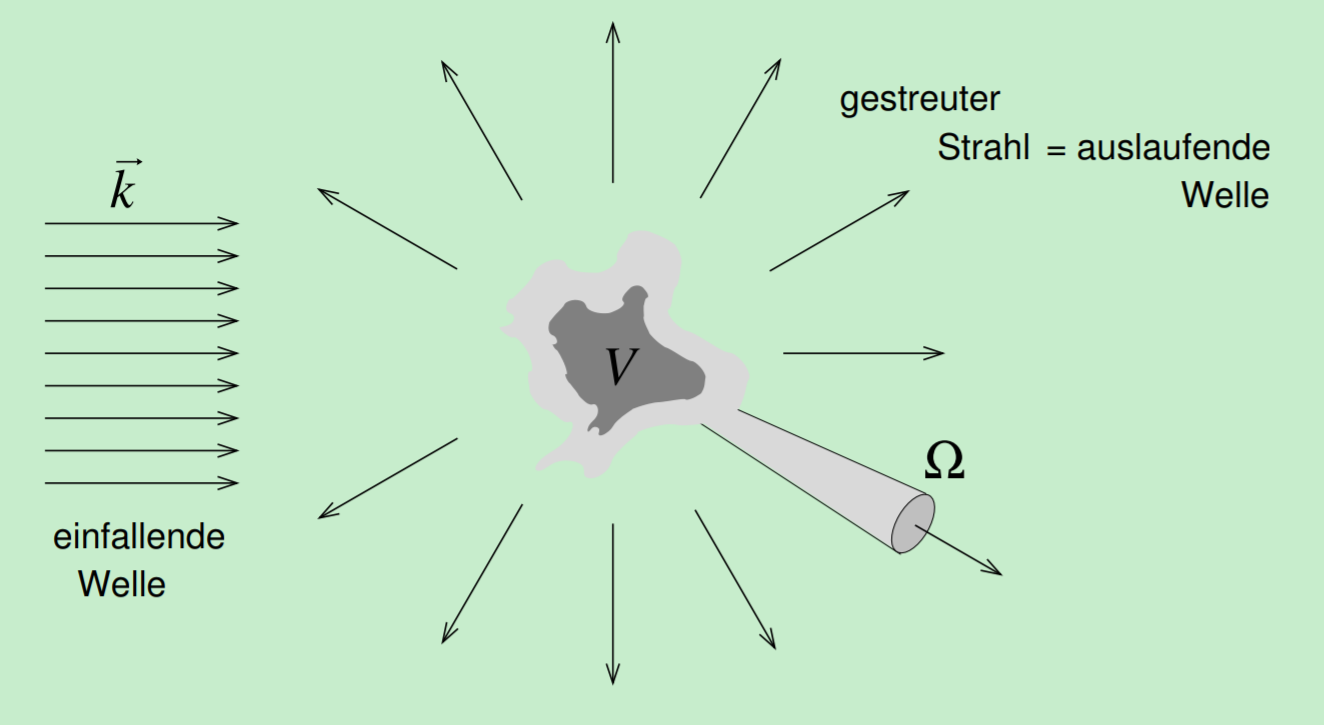
\includegraphics[scale=1]{6_1.PNG}
        \captionsetup{font={Large}}
        \caption{Scattering geometry: The incident wave $\operatorname{exp}(i\vec{k}\cdot\vec{r})$ is scattered by the potential $V(\vec{r})$. Asymptotically, the scattered wave has the form of a spherical wave $f_k(\Omega)\operatorname{exp}(ikr)/r$ modulated in the solid angle w.}
\end{figure}
\\
\section{Lippmann-Schwinger equation}
In a first step, we solve the eigenvalue problem (6.1) with the boundary condition (6.2),
%公式 6.3
\begin{equation}
    \underbrace{\left[\frac{\hbar^{2}}{2 m} \vec{\nabla}^{2}+E_{k}\right]}_{\text {freie Propagation }} \Psi_{\vec{k}}(\vec{r})=\underbrace{V(\vec{r}) \Psi_{\vec{k}}(\vec{r})}_{\text {Quelle }}
    \end{equation}
where we have already made a meaningful grouping of the terms, which is adapted to the scattering geometry. (6.3) is not an EW-problem in the usual sense (where $E_k$ is unknown): every energy $E_k$ produces a solution. (6.3) is an inhomogeneous partial differential equation, where the source $V(\vec{r})\Psi_{\vec{k}}(\vec{r})$ depends on the solution. Such driven differential equations are usually solved using Green's functions: We choose a point source $\delta(\vec{r})$ and solve
%公式 6.4
\begin{equation}
    \left[\frac{\hbar^{2}}{2 m} \nabla^{2}+E\right] G(\vec{r}, E)=\delta(\vec{r}) \quad \& \quad \text { Randbedingungen }(\mathrm{RB}) \text { für } G
    \end{equation}
If we know the solution (6.4) we can write the solution to (6.3) as
%公式 5
\begin{equation}
    \Psi_{\vec{k}}(\vec{r})=\underbrace{e^{i \vec{k} \cdot \vec{r}}}_{\text {Lösung der hom. Gl. }}+\underbrace{\int d^{3} r^{\prime} G\left(\vec{r}-\vec{r}^{\;\prime}, E_{k}\right) V\left(\vec{r}^{\;\prime}\right) \Psi_{\vec{k}}\left(\vec{r}^{\;\prime}\right)}_{\text {Lösung der inhomogenen Gleichung. }}
    \end{equation}
The solution of the homogeneous equation is just the incident wave and the solution of the inhomogeneous equation is the scattered wave. To prove that the integral equation (6.5) is equivalent to the problem (6.3) plus boundary conditions, we define the 'free' Hamiltonian $H_0 \equiv p^2 / 2m$ and apply the operator $(E_k - H_0)$ to (6.5),

%公式 6
\begin{equation}
\begin{aligned}\left(E_{k}-H_{0}\right) \Psi_{\vec{k}} &=\int d^{3} r^{\prime}\left[\left(E_{k}-H_{0}\right) G\left(\vec{r}-\vec{r}^{\;\prime}\right)\right] V\left(\vec{r}^{\;\prime}\right) \Psi_{\vec{k}^{\prime}}\left(\vec{r}^{\;\prime}\right) \\ &=\int d^{3} r^{\prime}\left[\delta\left(\vec{r}-\vec{r}^{\;\prime}\right)\right] V\left(\vec{r}^{\;\prime}\right) \Psi_{\vec{k}}\left(\vec{r}^{\;\prime}\right) \\ &=V(\vec{r}) \Psi_{\vec{k}}(\vec{r}) \end{aligned}
\end{equation}
The incident wave satisfies the first term of the asymptotic (6.2), the scattered wave must therefore give the second term $\propto exp (ikr) / r, r \rightarrow\infty$, in the asymptotic (6.2), for which we have the asymptotics of the Green's function G (cf. ~ r, E) need. We find the Green's function $G (\vec{r}, E)$ to be (6.4), $(E - H_0) G = \delta$, by Fourier transformation,
%公式 7
\begin{equation}
\begin{array}{c}{\int d^{3} r \mathrm{e}^{-i \vec{q} \cdot \vec{r}}\left(E-H_{0}\right) G(\vec{r}, E)=\int d^{3} r \delta^{3}(\vec{r}) e^{-i \vec{q} \cdot \vec{r}}} \\ {\left(E-\frac{\hbar^{2} q^{2}}{2 m}\right) G(\vec{q}, E)=1}\end{array}
\end{equation}

%公式 8
\begin{equation}
    G(\vec{q}, E)=\frac{1}{E-\hbar^{2} q^{2} / 2 m}=\frac{1}{E-\varepsilon_{q}}
    \end{equation}
By return transformation we get
%公式 9
\begin{equation}
\begin{aligned} G(\vec{r}, E) &=\int \frac{d^{3} q}{(2 \pi)^{3}} \frac{e^{i \vec{q} \cdot \vec{r}}}{E-\varepsilon_{q}} \\ &=-\frac{2 m}{\hbar^{2}} \int_{0}^{\infty} \frac{q^{2} d q}{4 \pi^{2}} \int_{-1}^{1} d z \frac{e^{i q z r}}{q^{2}-2 m E / \hbar^{2}} \\ &=-\frac{2 m}{4 \pi^{2} \hbar^{2}} \int_{0}^{\infty} d q q^{2} \frac{2 \sin q r}{q r} \frac{1}{q^{2}-2 m E / \hbar^{2}} \\ &=-\frac{m}{2 \pi^{2} \hbar^{2} i r} \int_{-\infty}^{\infty} d q \frac{q e^{i q r}}{q^{2}-2 m E / \hbar^{2}} \end{aligned}
\end{equation}
The last integral we can solve with the help of the residual theorem; In doing so, we implement the right boundary conditions, or in other words, we fix the analytic properties of $G (E, \vec{r})$. The integrand of (6.9) has poles at $q = \pm \sqrt{2mE }/ \hbar$. It is $r> 0$, so we have to conclude the integration path above, $i (q_r + iq_i) r = iq_rr - q_ir$ in the exponent. Further, we want an outgoing wave for $r\rightarrow\infty$, so we are interested in the pole at $+\sqrt{2mE} / \hbar$. We therefore choose the integration path $\gamma$ as appropriate
%图 6.2
\begin{figure}[ht]
    \begin{minipage}{0.5\textwidth}
        \centering
        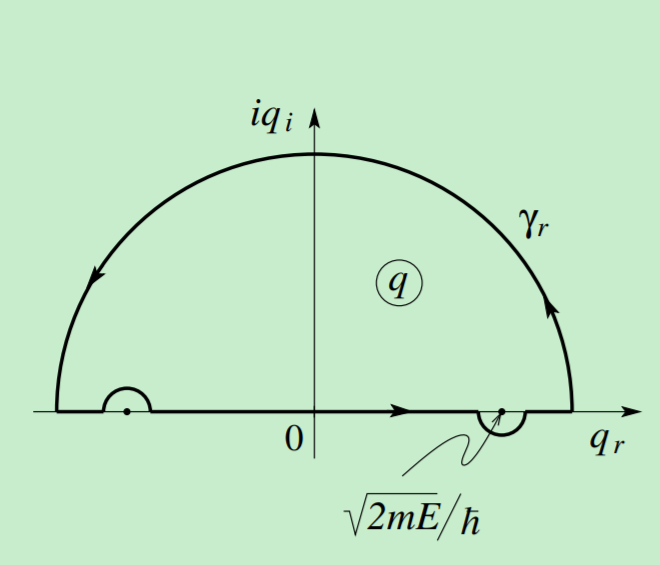
\includegraphics[scale=1]{6_2.PNG}
    \end{minipage}
    \begin{minipage}{0.5\textwidth}
        \captionsetup{font={Large}}
        \caption{Integration path in the complex $q$-plane. By including the pole at $q = + \sqrt{2mE} / \hbar$ we guarantee the asymptotics of an outgoing wave $\propto \operatorname{exp}[i(qr-ET\hbar)]$. The pole at $q = -\sqrt{2mE} / \hbar$ produces an incoming wave $\propto \operatorname{exp}[-i(qr+Et/\hbar)]$. The choice of the poles in the complex q-plane thus determines the RB.}
    \end{minipage}
\end{figure}
Figure 6.2 and received
%公式 10
\begin{equation}
    G(\vec{r}, E)=-\frac{m}{2 \pi \hbar^{2}} \frac{\mathrm{e}^{i \sqrt{2 m E} r / \hbar}}{r}
    \end{equation}
We can force the path $\gamma_r$ by itself by computing $G (\vec{r}, E + i\delta)$, the retarded Green's function: The denominator $q^2-2m (E + i\delta) / \hbar^2$ then has poles at $\pm p^2m (E + i\delta) / \hbar,$ see figure 6.3, and the integration over $¨ q \in \mathbb{R}$ automatically takes the pole at $+ \sqrt{2mE} / \hbar$. The choice $G^a (\vec{r}, E) \equiv G (\vec{r}, E - i\delta) = - (m / 2\pi\hbar^2)\operatorname{exp}[-i\sqrt{2mE}r/\hbar]/r$ produces an incident wave, so the choice $E = E + i\delta$ defines the boundary conditions and generates an outgoing wave (via the retarded Green's function $G^r$), conversely the choice $E - i\delta$ produces an incident wave (via the advanced Green's function Ga) With (6.10) we have found a formal solution of (6.3),
%图 6.3
\begin{figure}[ht]
    \begin{minipage}{0.5\textwidth}
        \centering
        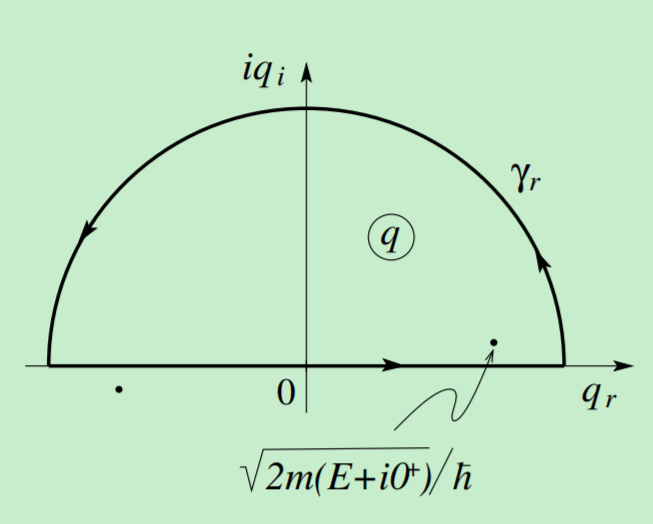
\includegraphics[scale=1]{6_3.PNG}
    \end{minipage}
    \begin{minipage}{0.5\textwidth}
        \captionsetup{font={Large}}
        \caption{By shifting the energy into the complex plane, $E\rightarrow E+i\delta$, the poles shift into the complex $q$-plane, $q=\pm\sqrt{2mE}/\hbar\rightarrow\pm \sqrt{2m(E+i\delta)}/\hbar$. The integration along $\mathbb{R}$ then automatically takes into account the right pole in the upper half-plane.}
    \end{minipage}
\end{figure}
%公式 11
\begin{equation}
\begin{aligned} \Psi_{\vec{k}}(\vec{r})=& e^{i \vec{k} \cdot \vec{r}}+\int d^{3} r^{\prime} G\left(\vec{r}-\vec{r}^{\;\prime}, E_{k}\right) V\left(\vec{r}^{\;\prime}\right) \Psi_{\vec{k}}\left(\vec{r}^{\;\prime}\right) \\ & \text { mit } \quad G\left(\vec{r}, E_{k}\right)=-\frac{m}{2 \pi \hbar^{2}} \frac{e^{i k r}}{r} \end{aligned}
\end{equation}
Of course, we have not really solved (6.3), we have just rewritten the differential equation into an integral equation, taking into account the boundary conditions. (6.11) is the Lippmann-Schwinger equation; it is physically transparent, automatically takes into account the boundary conditions and is well suited for implementing approximations.

Next, let us look at the distance range $r \rightarrow \infty$ in (6.11) to verify the asymptotic (6.2) and find an expression for $¨ f_k (\Omega)$ [depending on $V (\vec{r})$]. For $r\rightarrow\infty$ is $k|\vec{r}-\vec{r}^{\;\prime}|=kr\sqrt{(\hat{r}-\vec{r}^{\;\prime}/r)^2}=kr[1-2\hat{r}\cdot\vec{r}^{\;\prime}/r+(r^{\prime}/r)^2]^{1/2}\approx kr-\vec{k}_{\Omega}\cdot\vec{r}^{\;\prime}$ where $\vec{k}_{\Omega}=k\hat{r}$. This allows to transform (6.11)
%公式 12
\begin{equation}
    \Psi_{\vec{k}}(\vec{r}) \quad \rightarrow \quad e^{i \vec{k} \cdot \vec{r}}+\left[-\frac{m}{2 \pi \hbar^{2}} \int d^{3} r^{\prime} e^{-i \vec{k}_{\Omega} \cdot \vec{r}^{\;\prime}} V\left(\vec{r}^{\;\prime}\right) \Psi_{\vec{k}}\left(\vec{r}^{\;\prime}\right)\right] \frac{e^{i k r}}{r}
    \end{equation}
and we get the scattering amplitude in the form
%公式 13
\begin{equation}
    f_{k}(\Omega)=-\frac{m}{2 \pi \hbar^{2}} \int d^{3} r^{\prime} e^{-i \vec{k}_{\Omega} \cdot \vec{r}^{\;\prime}} V\left(\vec{r}^{\;\prime}\right) \Psi_{\vec{k}}\left(\vec{r}^{\;\prime}\right)
    \end{equation}
The scattering amplitude $f_k (\Omega)$ immediately gives us the differential cross section
%公式 14
\begin{equation}
\begin{aligned} 
    \frac{d \sigma}{d \Omega} & \equiv \frac{d i(\Omega)}{j_{\text {in }} d \Omega} \\ 
    &=\frac{\text { Zahl der in } d \Omega \text { gestreuten Teilchen pro sec }}{\text { einfallende Teilchen pro } \mathrm{cm}^{2} \text { und sec } \cdot d \Omega} \\
    [d \sigma / d \Omega] &=\mathrm{cm}^{2}, \text { barn } \quad 1 \text { barn }=10^{-24} \mathrm{cm}^{2} \end{aligned}
%
\end{equation}
Inserting the printouts for the incident and scattered current density,
%
$$
\begin{aligned} \vec{j}_{\mathrm{in}} &=\left.\frac{\hbar}{2 m i}\left(\Psi_{\mathrm{in}}^{*} \nabla \Psi_{\mathrm{in}}-c . c .\right)\right|_{\Psi_{\mathrm{in}}=e^{i \vec{k} \cdot \vec{r}} \cdot \vec{r}}=\frac{\hbar \vec{k}}{m} \\ j_{r} &=\left.\frac{\hbar}{2 m i}\left(\Psi_{s}^{*} \partial_{r} \Psi_{s}-c . c .\right)\right|_{\Psi_{s}=f_{k}(\Omega) e^{i k r} / r}=\frac{\hbar k}{m} \frac{1}{r^{2}}\left|f_{k}(\Omega)\right|^{2}+\mathcal{O}\left(r^{-3}\right) \end{aligned}
$$
$d i (\Omega) = j_rr^2d\Omega$ gives the differential cross section in the form
%
\begin{equation}
    \frac{d \sigma}{d \Omega}=\left|f_{k}(\Omega)\right|^{2}
    \end{equation}
Finally, we define the total cross section
%公式 16
\begin{equation}
    \sigma=\int d \Omega\left|f_{k}(\Omega)\right|^{2}
    \end{equation}
\section{Wave Packages}
We leave a wave packet (defined at time $t = t_0$)

%公式 17
\begin{equation}
    \Psi\left(\vec{r}, t_{0}\right)=\int \frac{d^{3} k}{(2 \pi)^{3}} a_{\vec{k}} e^{i \vec{k} \cdot \vec{r}}
    \end{equation}
come to the control center. The amplitude $a\vec{k}$ is concentrated around $\vec{k}_0$, so that the packet with velocity $\vec{v}_0=\hbar\vec{k}_0$ approaches the spreader. The time evolution of the wave function $\Psi(\vec{r},t)$ determines the signal measured in the detector at a later time $t> t_0$. Our task is thus to determine $\Psi (\vec{r}, t> t_0)$ at a later time. The scattering states $\Psi_{\vec{k}}$ are completely in the space of the extended wave functions and we can write the time evolution of $\Psi$ as
%
\begin{equation}
    \Psi(\vec{r}, t)=\int \frac{d^{3} k}{(2 \pi)^{3}} A_{\vec{k}} \Psi_{\vec{k}}(\vec{r}) e^{-i E_{k}\left(t-t_{0}\right) / \hbar}
    \end{equation}
At time t0, (6.17) and (6.18) must agree. We write (6.17) using (6.11) and then compare the coefficients
%公式 19
\begin{equation}
    \Psi\left(\vec{r}, t_{0}\right)=\int \frac{d^{3} k}{(2 \pi)^{3}} a_{\vec{k}}\left[\Psi_{\vec{k}}(\vec{r})+\frac{m}{2 \pi \hbar^{2}} \int d^{3} r^{\prime} \frac{e^{i k\left|\vec{r}-\vec{r}^{\;\prime}\right|}}{\left|\vec{r}-\vec{r}^{\;\prime}\right|} V\left(\vec{r}^{\;\prime}\right) \Psi_{\vec{k}}\left(\vec{r}^{\;\prime}\right)\right]
    \end{equation}
The scattering process is outlined in figure 6.4. In the second term we have to calculate the following expression
%公式 20
\begin{equation}
    \int \frac{d^{3} k}{(2 \pi)^{3}} a_{\vec{k}} e^{i k\left|\vec{r}-\vec{r}^{\;\prime}\right|} \Psi_{\vec{k}}\left(\vec{r}^{\;\prime}\right)
    \end{equation}
%图 6.4
\begin{figure}[ht]
        \centering
        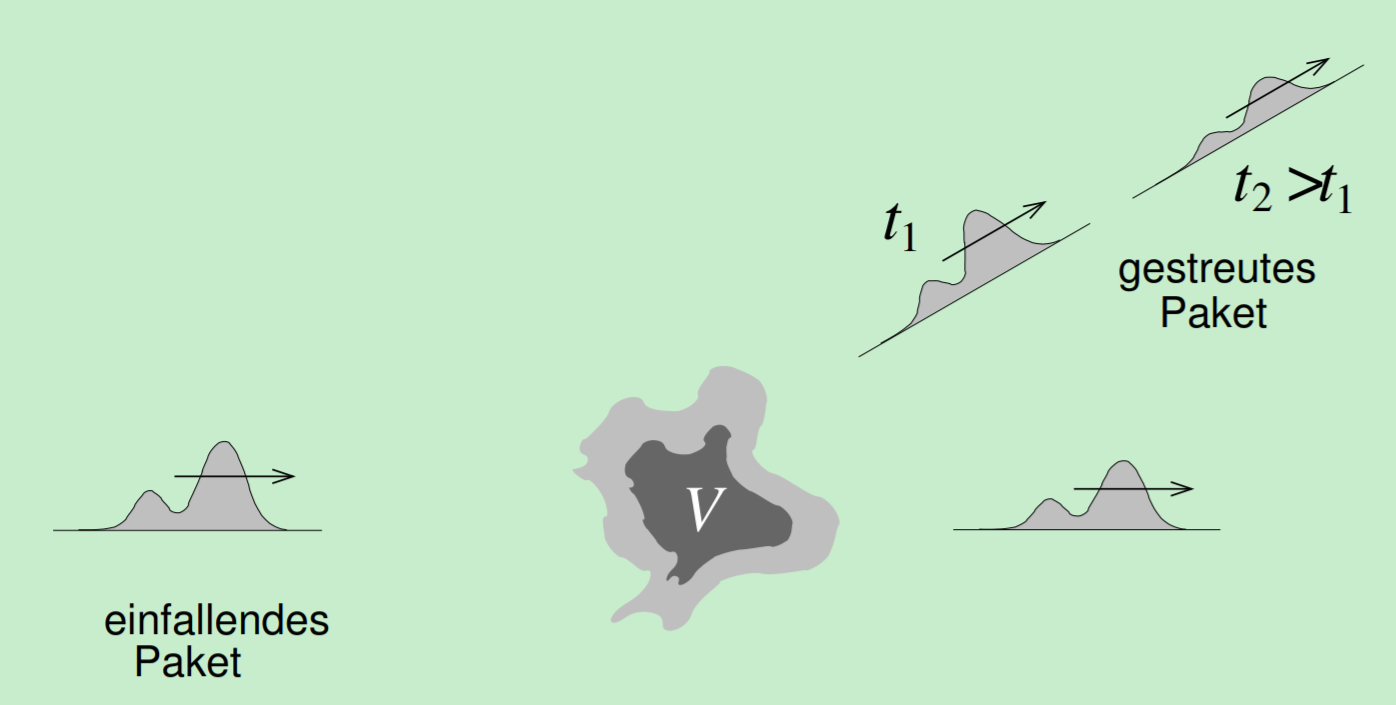
\includegraphics[scale=1]{6_4.PNG}
        \captionsetup{font={Large}}
        \caption{Scattering of a wave packet: The incoming packet is scattered with probability $\propto |f_{k_0}(\Omega)|^2$ in the direction w.}
\end{figure}
We assume that $\Psi_{\vec{k}}$ is smooth over the support of ¨$a_{\vec{k}}$, so has no resonance (see also later). Hence $\Psi_{\vec{k}}\approx\Psi_{\vec{k}_0}$ in (6.20). Further we can write $k$ as $k \approx \vec{k} \cdot\hat{k}_0$ and we get
%公式 21
\begin{equation}
    \int \frac{d^{3} k}{(2 \pi)^{3}} a_{\vec{k}} e^{i \vec{k} \cdot\left(\hat{k}_{0}\left|\vec{r}-\vec{r}^{\;\prime}\right|\right)} \Psi_{\vec{k}_{0}}\left(\vec{r}^{\;\prime}\right) \quad \stackrel{(6.17)}{=} \Psi\left(\hat{k}_{0}\left|\vec{r}-\vec{r}^{\;\prime}\right|, t_{0}\right) \Psi_{\vec{k}_{0}}\left(\vec{r}^{\;\prime}\right)
    \end{equation}
Here, $\Psi(\hat{k}_0|\vec{r}-\vec{r}^{\;\prime}|,t_0)$ evaluates the incident wave packet to the right of the scatterer, where it is by definition $\sim 0$. The expression (6.19) therefore has the form
%公式 22
\begin{equation}
    \Psi\left(\vec{r}, t_{0}\right)=\int \frac{d^{3} k}{(2 \pi)^{3}} a_{\vec{k}} \Psi_{\vec{k}}(\vec{r})
    \end{equation}
and the (coefficient) comparison with (6.18) yields $A_{\vec{k}}=a_{\vec{k}}$. Finally, we evaluate $\Psi (\vec{r}, t)$ at the detection time $t> t_0$ to understand that the above stationary analysis is really physically correct. According to (6.18)
%公式 23
\begin{equation}
\begin{aligned} \Psi(\vec{r}, t) &=\int \frac{d^{3} k}{(2 \pi)^{3}} a_{\vec{k}} \Psi_{\vec{k}}(\vec{r}) e^{-i E_{k}\left(t-t_{0}\right) / \hbar} \\ & \psi \stackrel{(6.12)(6.17)}{\longleftarrow} \\ & \sim \Psi_{0}(\vec{r}, t)+\int \frac{d^{3} k}{(2 \pi)^{3}} a_{\vec{k}} \frac{e^{i k r}}{r} f_{k}(\Omega) e^{-i E_{k}\left(t-t_{0}\right) / \hbar} \end{aligned}
\end{equation}
$\Psi_0(\vec{r},t)$ describes the evolution of the incoming packet without spreader,
%公式 24
\begin{equation}
    \Psi_{0}(\vec{r}, t)=\underbrace{\int \frac{d^{3} k}{(2 \pi)^{3}} a_{\vec{k}} e^{i \vec{k} \cdot \vec{r}} e^{-i E_{k}\left(t-t_{0}\right) / \hbar}}
    \end{equation}
With $f_k$ smooth around $\vec{k}=\vec{k}_0$ (with which one can draw $f_k \approx f_{k_0}$ in front of the integral) and $k\approx\vec{k}\cdot\hat{k}_0$ we obtain

%公式 25
\begin{equation}
    \Psi(\vec{r}, t) \stackrel{t \text { gross }}{\longrightarrow} \quad \underbrace{\Psi_{0}(\vec{r}, t)}_{\text {ungestreutes Wellenpaket }}+\underbrace{\frac{f_{k_{0}}(\Omega)}{r} \Psi_{0}\left(\hat{k}_{0} r, t\right)}_{\text {gestreutes Paket }}
    \end{equation}
The scattering process is sketched in figure 6.4: according to (6.25) it involves the superposition of the unscattered wave packet and a packet scattered in the direction of $\Omega$. The latter involves the amplitude $\Psi_0(\hat{k}_0r,t)$ of a packet propagating in the forward direction, which is to be evaluated only at the right time at the correct distance. This packet is then multiplied by the correct angle-dependent amplitude $f_{k_0}(\Omega)$; the angle thus appears only via the amplitude $f$ and not in the wave function $\Psi_0$. The above analysis is not applicable in two cases:
\begin{enumerate}
    \item[-] if $V$ is long-range, e.g., $V = 1 / r$,
    \item[-] if the incident energy $E_k$ is resonant.
\end{enumerate}


\section{Born approximation}
The Lippmann-Schwinger equation (6.11) and physical arguments suggest the following iteration scheme as a solution:
%公式 26
\begin{equation}
\begin{array}{c}{\Psi_{\vec{k}}=e^{i \vec{k} \cdot \vec{r}}+\int d^{3} r^{\prime} G\left(\vec{r}-\vec{r}^{\;\prime}, E_{k}\right) V\left(\vec{r}^{\;\prime}\right)  \Psi_{\vec{k}}\left(\vec{r}^{\;\prime}\right)} \\ {\downarrow} \\ {0^{\mathrm{te}} \text { Näherung }} \\ {\delta \Psi_{\vec{k}}^{(0)}(\vec{r})=e^{i \vec{k} \cdot \vec{r}}}\end{array}
\end{equation}
%公式 27
\begin{equation}
\begin{aligned} \delta \Psi_{\vec{k}}^{(1)}(\vec{r}) &=\int d^{3} r^{\prime} G\left(\vec{r}-\vec{r}^{\;\prime}, E_{k}\right) V\left(\vec{r}^{\;\prime}\right) \overbrace{e^{i\vec{k}\cdot\vec{r}^{\;\prime}}}^{\delta\Psi_{\vec{k}}^{(0)}(\vec{r}^{\;\prime})} \\ & \vdots \\ \delta \Psi_{\vec{k}}^{(n)}(\vec{r}) &=\int d^{3} r^{\prime} G\left(\vec{r}-\vec{r}^{\;\prime}, E_{k}\right) V\left(\vec{r}^{\;\prime}\right) \delta \Psi^{(n-1)}_{\vec{k}}\left(\vec{r}^{\;\prime}\right) \\ \rightarrow \Psi_{\vec{k}}^{(N)}(\vec{r}) &=\sum_{n=0}^{N} \delta \Psi_{\vec{k}}^{(n)}(\vec{r}) \end{aligned}
\end{equation}
For ¨$N <\infty$, (6.27) is the Nte Born approximation, the limit $N \rightarrow\infty$ yields the Born series. Mostly only the first Bornian approximation,

%公式 28
\begin{equation}
    \Psi_{\vec{k}}^{(1)}(\vec{r})=e^{i \vec{k} \cdot \vec{r}}+\int d^{3} r^{\prime} G\left(\vec{r}-\vec{r}^{\;\prime}, E_{k}\right) V\left(\vec{r}^{\;\prime}\right) e^{i \vec{k} \cdot \vec{r}^{\;\prime}}
    \end{equation}
second hand. For the scattering amplitude ¨$f_k^{(1)}(\Omega)$ we find
%公式 29
\begin{equation}
    f_{k}^{(1)}(\Omega)=-\frac{m}{2 \pi \hbar^{2}} \int d^{3} r^{\prime} V\left(\vec{r}^{\;\prime}\right) e^{i\left(\vec{k}-\vec{k}_{\Omega}\right) \cdot \vec{r}^{\;\prime}}
    \end{equation}
with $\vec{k}_{\Omega}=k\hat{e}_{\Omega}$, where $\hat{e}_\Omega$ denotes the unit vector in the direction of the solid angle $\Omega$. $f^{(1)}_k (\Omega)$ is given by the Fourier transform $V_{\vec{k}_{\Omega}-\vec{k}}$ of the scattering potential
\\\\
The validity of the approximation needs to be assessed on a case-by-case basis. Certainly it is necessary that $| \delta\Psi^{(1)} (\vec{r}) | <| \delta\Psi^{(0)} (\vec{r}) | = 1$, so
%
\begin{equation}
    \left|\frac{m}{2 \pi \hbar^{2}} \int d^{3} r^{\prime} V\left(\vec{r}^{\;\prime}\right) \frac{e^{i k\left|\vec{r}-\vec{r}^{\;\prime}\right|}}{\left|\vec{r}-\vec{r}^{\;\prime}\right|} e^{i \vec{k} \cdot \vec{r}^{\;\prime}}\right| \ll 1
    \end{equation}
For large particle energies and weak scattering potential, ¨$V_0 r_0k \ll E_k$, (where $V_0$ denotes the strength and r0 the extent of $V)$, the Born approximation is trustworthy: We set ¨ $\vec{r} = 0$ (this is the worst case) and take $V (\vec{r}) \sim V (r)$, then $| \delta\Psi^{(1)} (\vec{r}) |$ Write as
%公式
$$
    \frac{m}{2 \pi \hbar^{2}}\left|\int d^{3} r^{\prime} \frac{V\left(r^{\prime}\right)}{r^{\prime}} e^{i k r^{\prime}\left(1+\cos \vartheta^{\prime}\right)}\right|=\frac{m}{\hbar^{2} k}\left|\int_{0}^{\infty} d r^{\prime} V\left(r^{\prime}\right)\left(e^{2 i k r^{\prime}}-1\right)\right|
$$
For $kr_0\gg 1$ and $V$ smooth, the factor $\propto\operatorname{exp} (2ikr')$ is averaged out and we get $V (r) \sim V_0$
%公式 31
\begin{equation}
    \left|\frac{m}{\hbar^{2} k} \int_{0}^{\infty} d r V(r)\right| \ll 1 \rightarrow V_{0} r_{0} \ll \frac{\hbar^{2} k}{m}
    \end{equation}
Problematic are small energies $kr_0\ll 1$. With $\operatorname{exp} (2ikr' - 1) \sim 2ikr'$ we obtain the condition
%公式 32
\begin{equation}
    \left|\frac{m}{\hbar^{2}} \int_{0}^{\infty} d r r V(r)\right| \ll 1 \rightarrow V_{0} r_{0}^{2} \ll \frac{\hbar^{2}}{m}
    \end{equation}
that is, $V_0 \ll \hbar^2 / mr^2_0$, which corresponds to a flat potential (a corresponding attractive flat potential has no bound states).

\section{Rotationally symmetric potentials $V (r)$}
For rotationally symmetric scattering potentials ¨$V (r)$ the Hamiltonian $H = p^2 / 2m + V (r)$ commutes with the rotation operators $U_{\vec{w}} = \operatorname{exp} (-i \vec{w} \cdot L / \hbar), \vec{w} =$ rotation vector, $[H,U_{\vec{w}}] = 0$. Consequently, the angular problem can be separated and we can decompose the scattering problem according to the irreducible representations of the rotation group. This partial wave decomposition reduces the problem to the solution of the sub-problems in the different angular momentum sectors \footnote{The $2l + 1$ dimensional Hilbert space $\mathcal{H}_l = \{Y_{lm}\}^{m = l}_{m = -l}$ is spanned by the spherical functions to $l$}: We decompose the total silver space $\mathbb{L}_2 (\mathbb{R}^3)$ according to $\mathbb{L}_2 (\mathbb{R}^3) = \mathbb{L}_2 (\mathbb{R}^+) \bigotimes [\bigoplus_l\mathcal{H}_l]$ and solve the partial problems in $\mathbb{L}_2 (\mathbb{R}^+) \bigotimes \mathcal{H}_l$, where the angular problem is trivial (ie, already diagonalized). We fully exploit the rotational symmetry by choosing a coordinate system $\hat{e}_z || \vec{k}$ with the $z$-axis parallel to the incident beam, $\hat{e}_z||\vec{k}$. The whole problem is then rotationally symmetric with respect to rotations about the $z$-axis and only quantum numbers $m = 0$ occur. We can develop the required stationary solution in partial waves,
%公式 33
\begin{equation}
    \Psi_{\vec{k}}(\vec{r})=\sum_{l} i^{l}(2 l+1) \underbrace{P_{l}(\cos \theta)}_{\alpha Y_{l 0}} R_{l}(r)
    \end{equation}
where the factor $i^l (2l + 1)$ is an advantageous convention. If we substitute the theorem (6.33) into the stationary Schr¨odinger equation $H\Psi_{\vec{k}} = E_k\Psi_{\vec{k}}$, we obtain the radial problem (see 5.10).
%公式 34
\begin{equation}
    \left[-\frac{p_{r}^{2}}{2 m}-\frac{\hbar^{2} l(l+1)}{2 m r^{2}}+\frac{\hbar^{2} k^{2}}{2 m}\right] R_{l}(r)=V(r) R_{l}(r)
    \end{equation}
with $p_r^2/\hbar^2=-r^{-1}\partial_r^2 r$ this leads to the problem
%公式 35
\begin{equation}
    \left[\partial_{r}^{2}-\frac{l(l+1)}{r^{2}}+k^{2}\right] r R_{l}(r)=\frac{2 m}{\hbar^{2}} r V(r) R_{l}(r)
    \end{equation}
where $\Psi_{\vec{k}}$ has to satisfy the boundary conditions (6.2). In fact, the incident wave exp$ (i \vec{k}\cdot\vec{r})$ can be decomposed into partial waves: with the incident beam along the $z$-axis, $\vec{k} = (0, 0, k)$ and with $V = 0$ the spherical Bessel functions $R_l = j_l$ (see (5.23)) become regular solutions. They combine to the incident wave exp$(ikz) =$ exp$(ikr cos \theta)$ according to \footnote{
The approach


%公式 36
\begin{equation}
    e^{i k r \cos \theta}=\sum_{l} A_{l} j_{l}(k r) \underbrace{\sqrt{\frac{2 l+1}{4 \pi}} P_{l}(\cos \theta)}_{Y_{l 0}}
    \end{equation}
separates the radial and angular dependence in the incident wave function exp$ (i\vec{k}\cdot\vec{r})$; we have to determine the coefficients ¨ $A_l$. With (4.61), $P_l \perp P_{l'}$, we obtain by integration
%公式 37
\begin{equation}
    A_{l} j_{l}(k r)=\frac{1}{2} \sqrt{4 \pi(2 l+1)} \int_{-1}^{1} d z P_{l}(z) e^{i k r z}
    \end{equation}
We choose $r \rightarrow 0$, once develop exp$ (ikrz)$ on the right and $j_l (kr)$ on the left and compare the resulting coefficients. First the right side: We develop exp$ (ikrz)$ and get
%公式 38
\begin{equation}
    \int_{-1}^{1} d z P_{l}(z) \sum_{s=0}^{\infty} \frac{(i k r z)^{s}}{s !} \approx \int_{-1}^{1} d z P_{l}(z) \frac{(i k r z)^{l}}{l !}
    \end{equation}
where we have used that in the limiting case smaller $r$ only the term $s = l$ yields a noteworthy contribution (terms with $s <l$ do not contribute since $P_{l <s} \perp z^s=\Sigma_i a_iP_{i\leq s}$, terms with $s> l$ give a small correction). Next we replace $z^l$ by Legendre polynomials $P_{l'}(z)$ with $l' ≤ l$. Under the integral, terms vanish with $l' <l$ (orthogonality of the Legendre polynomials) and we can replace $(ikrz)^l/l!\rightarrow[(ikr)^l 2^l l! / (2l)!] P_l (z)$. Finally, we use the normalization of $P_l (z)$ to that Integral over $¨z$ to execute and receive
%公式 39
\begin{equation}
    \int_{-1}^{1} d z P_{l}(z) \sum_{s=0}^{\infty} \frac{(i k r z)^{s}}{s !} \approx \frac{(i k r)^{l} 2^{l+1} l !}{(2 l+1) !}
    \end{equation}
To the left: the evolution for $¨j_l$ gives $A_l j_l (kr) = [2^l l! / (2l + 1)!] (Kr)^lA_l$ (see (5.27)) and the coefficient comparison gives us the desired result.
}
%
\begin{equation}
    e^{i k r \cos \theta}=\sum_{l=0}^{\infty} i^{l}(2 l+1) j_{l}(k r) P_{l}(\cos \theta)
    \end{equation}
For the general case with $\vec{k}$ and $\vec{r}$ arbitrary we can use the addition theorem for $¨ Y_{lm}$ and print out $P_l (cos \theta)$ by the spherical functions, see (4.54); This gives us the expression for the plane wave
%公式 41
\begin{equation}
    e^{i \vec{k} \cdot \vec{r}}=4 \pi \sum_{l=0}^{\infty} \sum_{m=-l}^{l} i^{l} j_{l}(k r) Y_{l m}^{*}\left(\Omega_{\vec{k}}\right) Y_{l m}\left(\Omega_{\vec{r}}\right)
    \end{equation}
We now use the result (¨ 6.40) to find the boundary conditions for the radial waves $R_l (r)$. For $r \rightarrow\infty$, $V (r) \rightarrow 0$ (even $rV (r) \rightarrow 0$ goes by assumption) and $ R_l (r)$ must be asymptotic in shape

%
\begin{equation}
    R_{l}(r) \sim \alpha_{l}\left[h_{l}^{(2)}(k r)+s_{l} h_{l}^{(1)}(k r)\right]
    \end{equation}
With
%公式 43
\begin{equation}
    h_{l}^{(1,2)}(\rho) \sim \frac{1}{\rho} \exp [\pm i(\rho-(l+1) \pi / 2)], \quad \rho=k r
    \end{equation}
the two fundamental solutions for $¨V = 0$, the incoming and outgoing spherical waves in the form of Hankel functions (5.30). We have to determine the coefficients αl and sl; for ¨$V \equiv 0$ is obvious
%公式 44
\begin{equation}
    R_{l}(r)=j_{l}(k r)=\frac{1}{2}\left[h_{l}^{(2)}(k r)+h_{l}^{(1)}(k r)\right]
    \end{equation}
and thus $\alpha_l = 1/2, s_l = 1$. For ¨$V \neq 0$, the incident wave $h_l^{(2)}$ changes slightly, but the outgoing component $h^{(1)}_l$ changes, which is why the latter is a non-trivial weight $s_l \neq 1$ gets. The conservation of the particle number requires that $| s_l | = 1$ is: The total radial current density is (note that $\int dzP^2_l (z) = 2 / (2l + 1)$)

%公式 45
\begin{equation}
\begin{aligned} j_{r}^{l}(r) &=\frac{\hbar}{2 i m}\left[R_{l}^{*} \partial_{r} R_{l}-R_{l} \partial_{r} R_{l}^{*}\right] \\ & \downarrow 2 R_{l} \sim\left[e^{-i\left(k r+w_{l}\right)} / k r+s_{l} e^{i\left(k r+w_{l}\right)} / k r\right] \\ & \sim \frac{\hbar}{4 m k r^{2}}\left[\left|s_{l}\right|^{2}-1\right]=0 \end{aligned}
\end{equation}
because as many particles as possible come in and out. We can then use the amplitude $s_l$ as a complex phase
%
\begin{equation}
    s_{l}=e^{2 i \delta_{l}(k)}
    \end{equation}
write with the scattering phase $\delta_l (k)$. The scattering phase $\delta_l$ determines the solution of the scattering problem by specifying the scattering amplitude $f_k (\Omega)$: let's put the solution (6.33) in the asymptotic range

%公式 47
\begin{equation}
    \Psi_{\vec{k}}(\vec{r}) \sim \frac{1}{2} \sum_{l} i^{l}(2 l+1) P_{l}(\cos \theta)\left[h_{l}^{(2)}(k r)+e^{i 2 \delta_{l}} h_{l}^{(1)}(k r)\right]
    \end{equation}
with the help of (6.40) on the form (6.2)
%公式 48
\begin{equation}
    \Psi_{\vec{k}}(\vec{r}) \sim e^{i \vec{k} \cdot \vec{r}}+\underbrace{\frac{1}{2} \sum_{l} i^{l}(2 l+1) P_{l}(\cos \theta)\left[e^{2 i \delta_{l}}-1\right] h_{l}^{(1)}(k r)}_{\sim f_{k}(\theta) e^{i k r} / r}
    \end{equation}
Thus we obtain the scattering amplitude in the form $[h_l^{(1)}\sim(-i)^{l+1}e^{ikr}/kr]$

%公式 49
\begin{equation}
\begin{aligned} f_{k}(\theta) &=\frac{1}{2 i k} \sum_{l}(2 l+1) P_{l}(\cos \theta)\left[e^{2 i \delta_{l}}-1\right] \\ &=\frac{1}{k} \sum_{l}(2 l+1) P_{l}(\cos \theta) e^{i \delta_{l}} \sin \delta_{l} \end{aligned}
\end{equation}
We call
%公式 50
\begin{equation}
    \frac{e^{2 i \delta_{l}}-1}{2 i k}=\frac{e^{i \delta_{l}} \sin \delta_{l}}{k} \equiv f_{l}
    \end{equation}
the partial wave amplitude. To compute this, we must know the radial function $R_l (r)$: Starting from the equation (6.13) for $kf_k (\theta)$ we use the expression (6.33) for $\Psi_{\vec{k}}$ and (6.41) by the factor exp$ (- i\vec{k}_{\Omega} \cdot\vec{r}')$ in spherical coordinates,
%公式 51
\begin{equation}
\begin{aligned} f_{k}(\theta)=&-\frac{m}{2 \pi \hbar^{2}} \int d^{3} r^{\prime} e^{-i \vec{k}_{\Omega} \cdot \vec{r}^{\;\prime}} V\left(\vec{r}^{\;\prime}\right) \Psi_{\vec{k}}\left(\vec{r}^{\;\prime}\right) \\=&-\frac{m}{2 \pi \hbar^{2}} 4 \pi \sum_{l, l^{\prime}, m^{\prime}} \int d^{3} r^{\prime}(-i)^{l^{\prime}} j_{l^{\prime}}\left(k r^{\prime}\right) Y_{l^{\prime} m^{\prime}}(\Omega) Y_{l^{\prime} m^{\prime}}^{*}\left(\Omega^{\prime}\right) \\ & \times V\left(r^{\prime}\right) i^{l}(2 l+1) P_{l}\left(\cos \theta^{\prime}\right) R_{l}\left(r^{\prime}\right) \end{aligned}
\end{equation}
With $P_l (cos \theta')=\sqrt{4\pi/(2l+1)}Y_{l0}(\Omega')$ the integration over $ ¨d\Omega'$ gives the factor $\sqrt{4\pi/(2l+1)}\delta_{ll'}\delta_{m'0}$ and we find the expression

%公式 52
\begin{equation}
    f_{k}(\theta)=-\frac{2 m}{\hbar^{2}} \sum_{l=0}^{\infty}(2 l+1) P_{l}(\cos \theta) \int_{0}^{\infty} d r^{\prime} r^{\prime 2} V\left(r^{\prime}\right) j_{l}\left(k r^{\prime}\right) R_{l}\left(r^{\prime}\right)
    \end{equation}
which we compare with (6.49), which gives the result for $¨f_l$ (or $\delta_l$),
%公式 53
\begin{equation}
    f_{l}=\frac{e^{i \delta_{l}} \sin \delta_{l}}{k}=-\frac{2 m}{\hbar^{2}} \int_{0}^{\infty} d r^{\prime} r^{\prime 2} V\left(r^{\prime}\right) j_{l}\left(k r^{\prime}\right) R_{l}\left(r^{\prime}\right)
    \end{equation}
The total cross section $\sigma$ is obtained by an angle integration,
%公式 54
\begin{equation}
\begin{aligned} \sigma &=\int d \Omega\left|f_{k}(\Omega)\right|^{2} \\ &=\frac{4 \pi}{k^{2}} \sum_{l}(2 l+1) \sin ^{2} \delta_{l}=4 \pi \sum_{l}(2 l+1)\left|f_{l}\right|^{2} \end{aligned}
\end{equation}
The size
%公式 55
\begin{equation}
    \sigma_{l}=\frac{4 \pi}{k^{2}}(2 l+1) \sin ^{2} \delta_{l}=4 \pi(2 l+1)\left|f_{l}\right|^{2}
    \end{equation}
means partial cross section. Obviously $\sigma_l ≤ 4\pi (2l + 1) / k^2$. The phase shift exp$ (2i \delta_l)$ can be interpreted in a simple way physically: Consider the function

%公式 56
\begin{equation}
\begin{aligned} e^{i \delta_{l}} j_{l}\left(k r+\delta_{l}\right) &=\frac{e^{i \delta_{l}}}{2}\left[h_{l}^{(1)}\left(k r+\delta_{l}\right)+h_{l}^{(2)}\left(k r+\delta_{l}\right)\right] \\ & \sim \frac{e^{i \delta_{l}}}{2}\left[\frac{(-i)^{l+1} e^{i\left(k r+\delta_{l}\right)}}{k r+\delta_{l}}+\frac{(+i)^{l+1} e^{-i\left(k r+\delta_{l}\right)}}{k r+\delta_{l}}\right] \\ & \stackrel{k>r d}{\sim}\left[h_{l}^{(2)}(k r)+e^{2 i \delta_{l}} h_{l}^{(1)}(k r)\right] \sim R_{l} \end{aligned}
\end{equation}
Let us now compare the case
%公式 57
\begin{equation}
    V \equiv 0: \quad R_{l}(r)=j_{l}(k r)
    \end{equation}
With
%公式 58
\begin{equation}
    V \not=0: \quad R_{l}(r) \sim e^{i \delta_{l}} j_{l}\left(k r+\delta_{l}\right)
    \end{equation}
thus we see that a positive phase shift $\delta_l> 0$ pulls the wave function `into potential', while a negative phase shift $\delta_l <0$ puts out the wave, as sketched in Figure 6.5.

\subsection{Optical theorem}
Consider the forward scattering amplitude $f (0)$, respectively its imaginary part,
%公式 59
\begin{equation}
\begin{aligned} \operatorname{Im} f(0) &=\left.\frac{1}{k} \sum_{l}(2 l+1) P_{l}(\cos \theta) \sin ^{2} \delta_{l}\right|_{\theta=0} \\ &=\frac{1}{k} \sum_{l}(2 l+1) \sin ^{2} \delta_{l}=\frac{k}{4 \pi} \underbrace{\frac{4 \pi}{k^{2}} \sum(2 l+1) \sin ^{2} \delta_{l}}_{\sigma} \end{aligned}
\end{equation}
%图 6.5
\begin{figure}[ht]
    \centering
    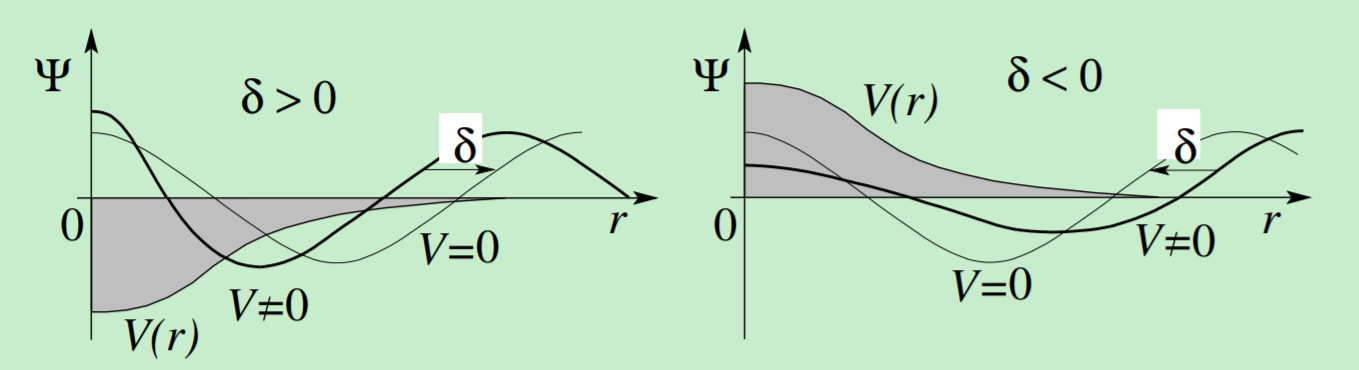
\includegraphics[scale=1]{6_5.PNG}
    \captionsetup{font={Large}}
    \caption{Phase shifts $\delta_l(k)$: An attractive potential (left) increases the kinetic energy and the wave function oscillates faster, which leads to a positive phase shift. Conversely, a repulsive potential (right) slows down the oscillation of the wave function and produces a negative $\delta_l(k)$.}
\end{figure}
We get the optical theorem
%公式 60
\begin{equation}
    \sigma=\frac{4 \pi}{k} \operatorname{Im} f(0)
    \end{equation}
The deeper cause of the optical theorem can be found in the conservation of the number of particles: The scattered particle flow $(\hbar k / m) \sigma = I_{Streu}$ must be taken from the incident current $I_0$ by scattering and thus lacks in the forward amplitude. It is the interference of the scattered wave with the incident wave that reduces the unscattered wave and thus creates a shadow of the scatterer in the forward direction. The missing particles in the shadow are just those which have been scattered $\leftrightarrow$ optical theorem (for details see Baym or Schwabel). Note that the relation (6.60) is generally valid as long as the particle number is conserved; this is the case when there is no capture and no conversion of the particles.

\subsection{Born approximation for $\delta_l (k)$}
A scattering problem can be considered to be solved if we know the scattering amplitude $f_k (\theta)$, since this gives us the current measured in the detector (the latter is the measuring magnitudes in the scattering problem). For $\mathcal{SO} (3)$ symmetric problems, $f_k$ is known as soon as we know the scattering phases $\delta_l (k)$. The latter must usually be found numerically by integration of the radial equation (¨ 6.34). We expect that only angular momenta $l<kr_0$ will suffer significant phase shifts, where $r_0$ represents the range of the potential. Particles with larger angular momenta have perturbation parameters $b \sim l / k$ which are outside the range $r_0$ of the potential. We see that thus $s$-waves always scatter, whereas $p$-waves (and higher angular momenta) are only weakly scattered at low energies $E <\hbar^2 / 2mr^2_0$. In these cases, we obtain an approximate calculation of $\delta_l$: Starting from (6.53) we replace the radial function $R_l (r)$ by the component $j_l (kr)$ of the incident wave and obtain


%公式 61
\begin{equation}
    f_{l}=\frac{e^{i \delta_{l}} \sin \delta_{l}}{k} \approx-\frac{2 m}{\hbar^{2}} \int_{0}^{\infty} d r r^{2} V(r) j_{l}^{2}(k r)
    \end{equation}
The result (6.61) is the Born approximation for the scattering phase $\delta_l (k)$. For large $l, j_l (r \rightarrow 0)$ is small, $j_l \sim r^l$, and δl becomes small for a bounded potential $V (r)$. Note that $R_l \approx j_l$ is not a good approximation in areas where $V$ is large and $R_l$ is strongly suppressed (e.g., a hard sphere).
\subsection{Analyticity of $s_l (E)$}
We consider a short-range potential which disappears outside of $r = r_0$. The radial solution for $r> r_0$ is then given by
%公式 62
\begin{equation}
    R_{l}(r)=\frac{1}{2}\left[h_{l}^{(2)}(k r)+s_{l} h_{l}^{(1)}(k r)\right]
    \end{equation}
whereas $R_l$ must be found for $r<r_0$ by integrating (6.34). The scattering phase $s_l$ must be set up in such a way that $R_l$ and $\partial_r R_l$ coincide at $r_0$ (continuity). The normalization factor drops out in the logarithmic derivative $(1 / R_l) \partial_rR_l = \partial_r \operatorname{ln} R_l$ and we use the boundary condition
%公式 63
\begin{equation}
    \alpha_{l}=\left.\frac{1}{R_{l}} \frac{\partial R_{l}}{\partial r}\right|_{r_{0}^{-}}=\left.\frac{\partial_{r} h_{l}^{(2)}+s_{l} \partial_{r} h_{l}^{(1)}}{h_{l}^{(2)}+s_{l} h_{l}^{(1)}}\right|_{r_{0}^{+}}
    \end{equation}
Resolutions after the scattering phase results

%公式 64
\begin{equation}
\begin{aligned} s_{l}-1 &=\left.\frac{2\left(\partial_{r}-\alpha_{l}\right) j_{l}}{\left(\alpha_{l}-\partial_{r}\right) h_{l}^{(1)}}\right|_{r_{0}} \\ & \downarrow \text { mit } s_{l}=1+\frac{2 i}{\cot \delta_{l}-i} \end{aligned}
\end{equation}
%公式 65
\begin{equation}
    \cot \delta_{l}=\left.\frac{\left(\partial_{r}-\alpha_{l}\right) n_{l}}{\left(\partial_{r}-\alpha_{l}\right) j_{l}}\right|_{r_{0}}
    \end{equation}
where $\delta_l$ follows from $\alpha_l$. The partial cross section is
%公式 66
\begin{equation}
    \sigma_{l}=\frac{4 \pi}{k^{2}}(2 l+1) \sin ^{2} \delta_{l}=\frac{4 \pi}{k^{2}} \frac{2 l+1}{1+\cot ^{2} \delta_{l}}
    \end{equation}
The analysis of the expressions for $s_l(\operatorname{cot} \delta_l)$ and $\sigma_l (\operatorname{cot}\delta_l)$ shows that the following statements hold: for
%公式 67
\begin{equation}
\begin{array}{ll}{\cot \delta_{l}=i} & {\text { has } s_{l} \text { a pole, } \sigma_{l} \text { is } \infty} \\ 
{\cot \delta_{l}=0} & {  \text { it is } s_{l}=-1 \text { and } \sigma_{l}=4 \pi(2 l+1) / k^{2} \text { is maximal. }}\end{array}
\end{equation}
As in dim = 1, the poles of $s_l$ correspond to just bound states: For a bound state, we have asymptotically $R_l(r)\sim h_l^{(1)}(i\kappa r)\propto e^{-\kappa r}$ with the binding energy $E_B = - \hbar^2\kappa^2 / 2m$ , The continuity condition is given by
%公式 68
\begin{equation}
    \alpha_{l}=\partial_{r} h_{l}^{(1)} /\left.h_{l}^{(1)}\right|_{r_{0}}=\left.\partial_{r} \ln h_{l}^{(1)}\right|_{r_{0}}
    \end{equation}
and insert into the general continuity condition (6.65)
%公式 69
\begin{equation}
    \cot \delta_{l}=\frac{h_{l}^{(1)} \partial_{r} n_{l}-n_{l} \partial_{r} h_{l}^{(1)}}{h_{l}^{(1)} \partial_{r} j_{l}-j_{l} \partial_{r} h_{l}^{(1)}} \quad^{h_{l}^{(1)}=j_{l}+i n_{l}} i
    \end{equation}
Likewise, the zeros of cot$\delta_l$ just correspond to the stray resonances: we evolve around the resonance,

%公式 70
\begin{equation}
\begin{aligned} \cot \delta_{l}(E) & \approx \cot \delta_{l}\left(E_{r}\right)-\left.\frac{1}{\sin ^{2} \delta_{l}} \frac{d \delta_{l}}{d E}\right|_{E_{r}}\left(E-E_{r}\right) \\ &=-\left.\frac{d \delta_{l}}{d E}\right|_{E_{r}}\left(E-E_{r}\right) \\ & \downarrow \text { mit: } \Gamma_{r}=\left.\frac{2}{\partial_{E} \delta_{l}}\right|_{E_{r}} \end{aligned}
\end{equation}
%公式 71
\begin{equation}
    \equiv-\frac{2}{\Gamma_{r}}\left(E-E_{r}\right)
    \end{equation}
This gives a resonance peak of width $\Gamma_r$ in the partial cross-section $\sigma_l$ with the shape
%公式 72
\begin{equation}
    \sigma_{l}=\frac{4 \pi}{k^{2}}(2 l+1) \frac{\left(\Gamma_{r} / 2\right)^{2}}{\left(E-E_{r}\right)^{2}+\left(\Gamma_{r} / 2\right)^{2}}
    \end{equation}
see figure 6.6. The scattering amplitude $s_l (E)$ has a pole in the 2nd Riemann plane of the complex energy plane,
%公式 73
\begin{equation}
    s_{l}-1=\frac{-i \Gamma_{r}}{E-\left(E_{r}-i \Gamma_{r} / 2\right)}
    \end{equation}
%图 6.6
\begin{figure}[ht]
    \centering
    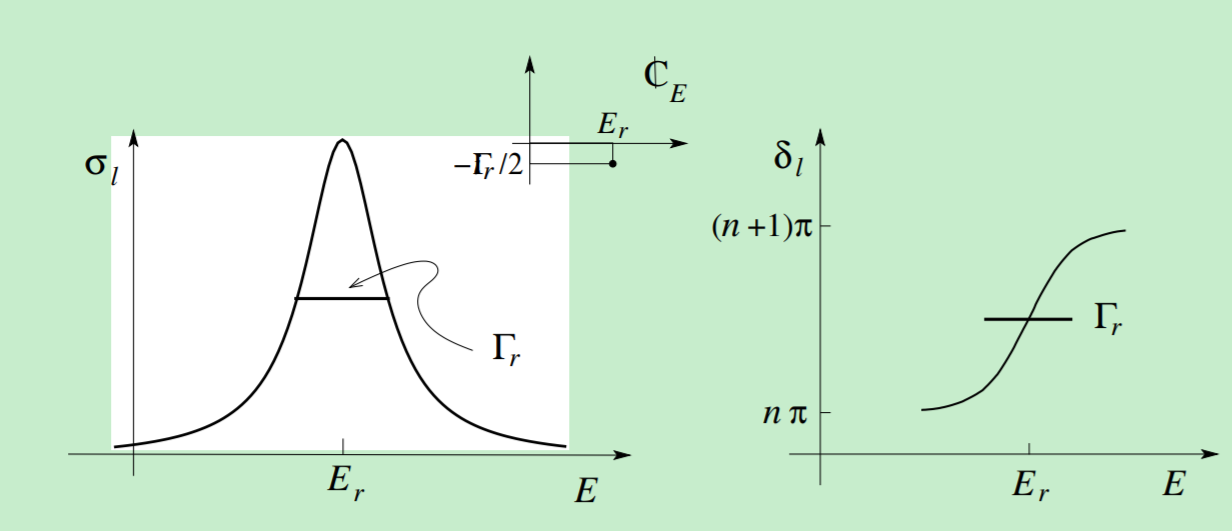
\includegraphics[scale=1]{6_6.PNG}
    \captionsetup{font={Large}}
    \caption{Resonance peak of width $\Gamma_r$: on the left the cross-section $\sigma_l(E)$ and on the right the scattering phase $\delta_l(E)$; in the middle the position of the pole is sketched in the complex $E$-plane.}
\end{figure}
the scattering phase $\delta_l (E)$ increases by $\pi$, the steeper the tighter the resonance. The value $\delta_l (E = 0)$ gives the number of bound states: it is $\delta_l (0) = n^l_{bound}\pi$, where an additional phase shift $+ \pi / 2$ occurs in the sector $l = 0$ if a 'virtual' state \footnote{Im $l = 0$ sector, a bound state at $E <0$ to a virtual state (instead of a resonance) when the binding energy disappears, ie, $E \rightarrow 0$} exists to $E = 0$, see Levinson's Theorem. 
\\\\
In the following we consider the deep-energy behavior $kr_0 \ll 1$ for a spreader of the expansion $r_0$ a little more accurately.

\subsection{Depth-Energy Scattering, $kr_0\ll 1$}
Low-energy scattering of atoms has recently become a very relevant topic in quantum atom optics (cold atomic gases). We use the developments $j_l \sim x^l / (2l + 1) !!$ and $n_l \sim - (2l - 1) !! / x^{l + 1}$ in (6.65) and get for ¨ $kr_0\ll 1$
%公式 74
\begin{equation}
    \cot \delta_{l} \approx \frac{(2 l+1) ! !(2 l-1) ! !}{\left(k r_{0}\right)^{2 l+1}} \frac{l !+r_{0} \alpha_{l}(E)}{l-r_{0} \alpha_{l}(E)}
    \end{equation}
A rough estimate shows that
%公式 75
\begin{equation}
\begin{aligned} \cot \delta_{l}=\frac{\cos \delta_{l}}{\sin \delta_{l}} & \approx \frac{1}{\sin \delta_{l}} \sim \frac{1}{\left(r_{0} k\right)^{2 l+1}} \\ & \rightarrow \sin \delta_{l} \sim\left(r_{0} k\right)^{2 l+1} \end{aligned}
\end{equation}
that is, the scattering phases $\delta_l$ become rapidly smaller in the low energy region as the angular momentum increases; the $l = 0$ sector is dominant and we focus on this case first. A more detailed analysis of the scattering phase $\delta_0$ leads these to just one parameter, the scattering $a$, back

%公式 76
\begin{equation}
    k \cot \delta_{0} \quad \approx^{\alpha_{0}(E)} \approx^{\alpha_{0}(0)} \quad-\frac{1+r_{0} \alpha_{0}(0)}{r_{0}^{2} \alpha_{0}(0)} \equiv-\frac{1}{a}
    \end{equation}
the scattering a is then the relevant parameter in the problem. For ¨ $\alpha_0r_0\gg 1,\text{ is } a \approx r_0$; for example, for the hard sphere ¨$R_l (r_0) = 0, \alpha_l = \infty, a = r_0> 0$ and cot$ \delta_0 = -1 / kr_0$. Therefore, for small $kr_0, \delta_0 ≈ -kr_0 <0$, resulting in a negative phase shift for the repulsive potential, as expected. The cross section $\sigma_0$ is

%公式 77
\begin{equation}
    \sigma_{0}=\frac{4 \pi}{k^{2}} \frac{1}{1+\cot ^{2} \delta_{0}} \approx \frac{4 \pi}{k^{2}+1 / a^{2}}
    \end{equation}
In comparison, the cross sections for higher angular momenta $\sigma_l \propto [\operatorname{sin}^2\delta_l] / k^2$ are correct
%公式 78
\begin{equation}
    \sigma_{l} \propto r_{0}^{2}\left(r_{0} k\right)^{4 l} \rightarrow 0
    \end{equation}
accordingly, we find that the depth-energy distribution has $s$-character and $\sigma$ is dominated by $\sigma_0$. In particular

%
\begin{equation}
    \sigma(E=0)=4 \pi a^{2}
    \end{equation}
for the hard sphere with $a = r_0$, we find a fourfold larger scattering cross-section than classically expected, $\sigma_{kl} = \pi r^2_0$.
Next, consider bound states and resonances in the s channel. The scattering phase can be written using the scattering $a$ as
%公式 80
\begin{equation}
    s_{0}-1=\frac{2 i}{\cot \delta_{0}-i} \approx \frac{2 k a}{i-k a}=\frac{2 \sqrt{E}}{\sqrt{E_{B}}-\sqrt{E}}
    \end{equation}
with the energy
%公式 81
\begin{equation}
    E_{B}=-\frac{\hbar^{2}}{2 m a^{2}}
    \end{equation}
a bound state. Note that we used that $| kr_0 |\ll 1$ and therefore $| k |\ll 1 / r_0$; with $| k | = 1 / a\ll 1 / r_0$, a weakly bound state produces a large positive scattering $a\gg r_0> 0$ in the problem -- a weakly bound state repels a low-energy scattering particle. The bound state can also be felt in the cross-section,

%公式 82
\begin{equation}
    \sigma \approx \sigma_{0} \approx \frac{2 \pi \hbar^{2} / m}{E-E_{B}}, \quad E_{B} \lesssim 0
    \end{equation}
For $E_B \rightarrow 0$ we get $a \rightarrow \infty, \sigma\rightarrow 4\pi a^2 \rightarrow \infty$ if $E \rightarrow 0$. Note that in the $s$-channel no bound state is possible at $E_B = 0$\footnote{Consider the radial differential equation $[\partial^2r - l (l + 1) / r^2 - U (r)] u (r) = 0$ to $E = 0$. With $E = 0$, the centrifugal m is dominant for $¨r \rightarrow 0$ and $r \rightarrow\infty$. For any potential $U (r)$ At $r \sim 0$, the regular solution $r^{l + 1}$ goes into a combination of the generic solutions $r^(l + 1)$ and $r^{-l}$, and is therefore not normable, for special potentials $¨U$ the $r$ vanishes $(l + 1)$ term for $r\rightarrow\infty$, the solution can be normalized, resulting in a bound state at $E = 0$. For $l = 0, r^{-l}$ does not decay and the state is not normalizable there is no bound state to $E = 0$ in the $l = 0$ sector.} instead, one finds a pseudoresonance for $¨ E_B = 0$ with infinite scattering cross section and infinite scattering.
s-channel resonances are obtained according to (6.74) if
%公式 83
\begin{equation}
    \cot \delta_{0}=0 \approx \frac{1}{k_{r} r_{0}} \frac{1+r_{0} \alpha_{0}\left(E_{r}\right)}{-r_{0} \alpha_{0}\left(E_{r}\right)}
    \end{equation}
and thus the condition must
%公式 84
\begin{equation}
    1+r_{0} \alpha_{0}\left(E_{r}\right) \approx 0
    \end{equation}
be satisfied. For a resonance, the condition $\Gamma_r <E_r$ also applies, which guarantees a (albeit broad) resonance maximum. With

%公式 85
\begin{equation}
\begin{aligned} \cot \delta_{0}(E) & \approx-\frac{2}{\Gamma_{r}}\left(E-E_{r}\right) \\ &=\frac{1}{k_{r} r_{0}} \frac{\overbrace{1+r_{0} \alpha_{0}\left(E_{r}\right)}+r_{0} \partial_{E} \alpha_{0}\left(E-E_{r}\right)}{\underbrace{-r_{0} \alpha_{0}\left(E_{r}\right)}}_{1} \end{aligned}
\end{equation}
we get the condition
%公式 86
\begin{equation}
    \Gamma_{r}=-\frac{2 k_{r} r_{0}}{r_{0} \partial_{E} \alpha_{0}}=-\frac{2 k_{r}}{\partial_{E} \alpha_{0}}<\frac{\hbar^{2} k_{r}^{2}}{2 m}=E_{r}
    \end{equation}
%公式 87
\begin{equation}
    \Rightarrow\left|\frac{\partial \alpha_{0}}{\partial k^{2}}\right|>\frac{2}{k_{r}}
    \end{equation}
for the formation of a resonance.
Next we investigate the case $l> 0$. In general, the scattering in the $l> 0$ channel is small: with sin$ \delta_l \propto (r_0k)^{2l + 1}$ we find
%公式 88
\begin{equation}
    \sigma_{l}=\frac{4 \pi}{k^{2}} \frac{(2 l+1)}{1+\cot ^{2} \delta_{l}}=\frac{4 \pi}{k^{2}}(2 l+1) \sin ^{2} \delta_{l} \propto r_{0}^{2}\left(r_{0} k\right)^{4 l} \stackrel{k \rightarrow 0}{\longrightarrow} 0
    \end{equation}
Near a resonance, cot$ \delta_l \sim 0$ and $\sigma_l$ goes through a maximum,
%公式 89
\begin{equation}
    \sigma_{l} \sim \frac{4 \pi}{k^{2}}(2 l+1)
    \end{equation}
By (6.74) we find resonances

%公式 90
\begin{equation}
    l+1+r_{0} \alpha_{l}\left(E_{r}\right) \approx 0
    \end{equation}

For the breadth of the resonance we get \footnote{
    We use the expression $l - r_0\alpha_l$ in
    %公式 91
\begin{equation}
    \cot \delta_{l} \approx \frac{(2 l+1) ! !(2 l-1) ! !}{\left(k r_{0}\right)^{2 l+1}} \frac{l+1+r_{0}\left(\alpha_{l}+\partial_{E} \alpha_{l}\left(E-E_{r}\right)\right)}{l-r_{0} \alpha_{l}}=-\frac{2}{\Gamma_{r}}\left(E-E_{r}\right)
    \end{equation}
    can be replaced by $2l + 1$.}
%公式 92
\begin{equation}
    \Gamma_{r}=-\frac{2 k\left(r_{0} k\right)^{2 l}}{[(2 l-1) ! !]^{2} \partial_{E} \alpha_{l}} \propto k^{2 l+1}
    \end{equation}
The smaller $k$ and the larger $l ≥ 1$, the sharper the resonance. It should be noted that $E_r\propto k^2$ but $\Gamma_r\propto k^3$ at least; for $¨ l = 0$ it disappears faster than $\Gamma_r$ and the size of $\partial_E\alpha_0$ must save the resonance, cf. (6.87). Likewise, the larger the resonance, the greater the resonance (so sharp resonances in $\delta_l$ also result).\\\\
$l> 0$ bound states we get again for cot$\delta_l = i$. In the lowest order, the condition for a weakly bound state is just equal to the resonance condition, $l + 1 + r_0\alpha_l (E_B <0) \approx 0$; only the consideration of terms of higher order in $kr_0$ in $\alpha_l (E)$ allows us to distinguish cot$\delta_l (E_B <0) = i$ for bound states and cot$\delta_l (E_r> 0) = 0$ for resonances.\footnote{For a resonance, $r_0\alpha_l = -l-1$. For the pole we have $i (r_0k)^{2l + 1} = \nu_l (l + 1 + r_0\alpha_l) / (l-r_0\alpha_l)$ with $\nu_l = (2l + 1) !! (2l - 1) !!$ a number.The left-hand side is small and therefore $r_0\alpha_l = -l -1 + r_0\delta\alpha_l$. Substituting in the equation for the pole yields $\delta\alpha_l (k) \approx ik (r_0k)^2l (2l + 1) / \nu_l$ as an equation for determining the position of the pole.}
\\\\
In summary, we find the following behavior for low-energy scattering $¨ E \rightarrow 0 (kr_0\ll 1)$:
%公式
$$
    \sigma \approx \sigma_{0}=\frac{4 \pi}{k^{2}+a^{-2}}, \quad \sigma(0)=4 \pi a^{2}, \quad \sigma_{l} \propto k^{4 l} \rightarrow 0
$$
%图 6.7
\begin{figure}[ht]
        \centering
        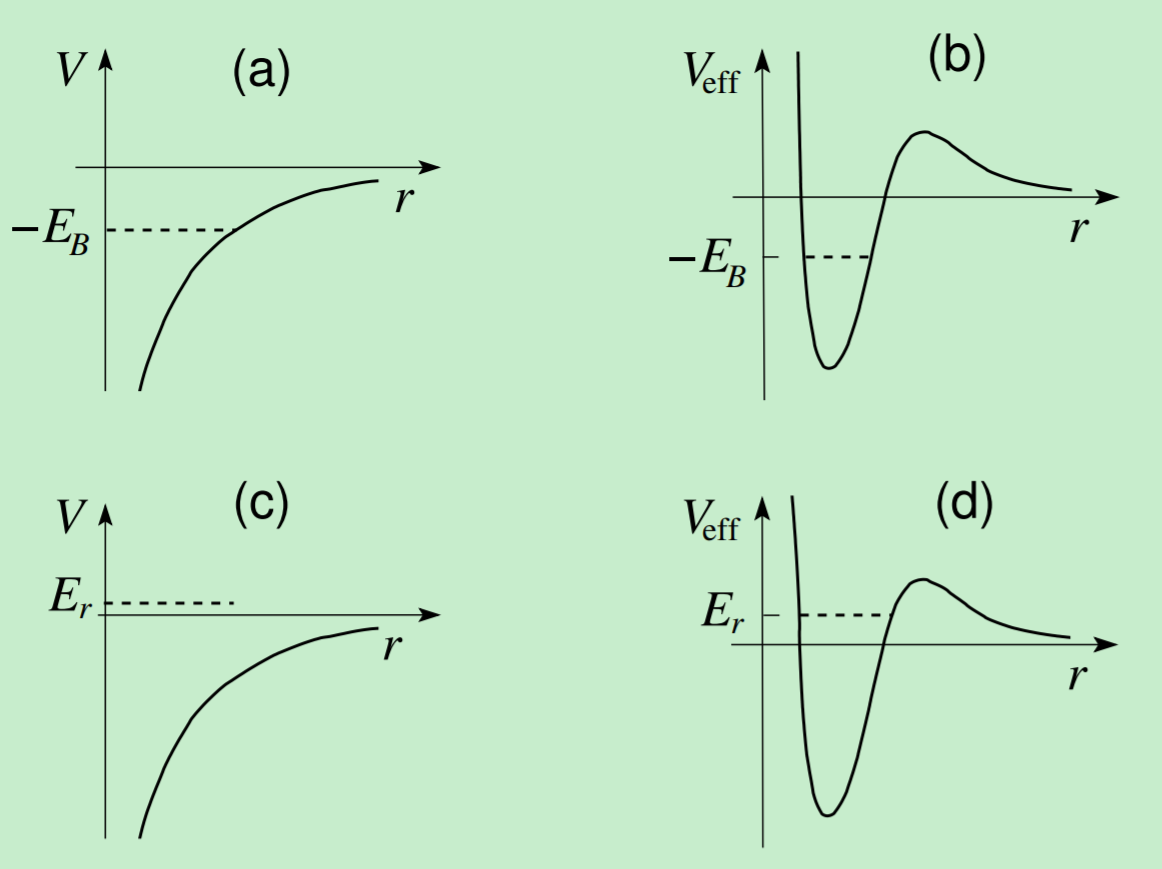
\includegraphics[scale=1]{6_7.PNG}
        \captionsetup{font={Large}}
        \caption{Bound states (a, b) and resonances (c, d): (a) Bound state for $l = 0$. (b) Bound state for> 1> 0, with the potential $V (r)$ replaced by the effective state Potential with centrifugal barrier $\hbar^2l (l +1) / 2mr^2$. (c) In the $l = 0$ sector, the resonances are broad, possibly undefined with $\Gamma_r> E_r$. A defined resonance with $\Gamma_r <E_r$ implies that $| \partial_E\alpha_0 |$ is big. (d) For $l> 0$, sharp resonances result, since the decay of the state is suppressed by the centrifugal barrier. The resonances are the sharper the smaller $k$, the larger $l$, and the larger $\partial_E\alpha_l$ are.}
\end{figure}
\subsection{Great energies $kr_0\gg 1$}
The angular momenta with $l \leq kr_0$ contribute strongly to $\sigma$ (parameter within $r_0$). For a hard sphere, $\alpha_l = \infty$ and cot$\delta_l = n_l (kr_0) / j_l (kr_0)$. With the help of the asymptotic for $¨j_l$ and $n_l$ we obtain cot$\delta_l \sim\operatorname{cot}(kr_0 - l\pi / 2), \delta_l \sim -cr_0 + l\pi / 2 (+ n\pi)$. With these scattering phases, we can calculate the cross-section,

%公式 93
\begin{equation}
\begin{aligned} \sigma & \approx \frac{4 \pi}{k^{2}} \sum_{l=0}^{k r_{0}}(2 l+1) \sin ^{2} \delta_{l} \\ &=\frac{4 \pi}{k^{2}} \sum_{l=0}^{k r_{0}}\left[(l+1) \cos ^{2}\left(k r_{0}-(l+1) \pi / 2\right)+l \sin ^{2}\left(k r_{0}-l \pi / 2\right)\right] \\ & \approx \frac{4 \pi}{k^{2}} \sum_{l=1}^{k r_{0}} l\left(\cos ^{2}+\sin ^{2}\right)=\frac{4 \pi}{k^{2}} \frac{k r_{0}\left(k r_{0}+1\right)}{2} \approx 2 \pi r_{0}^{2} \end{aligned}
\end{equation}
just twice as big as the classic result.

\section{Regge Poles \& Trajectors*}
According to the last section 6.4.3, page 182, we know that the scatter function
%公式 94
\begin{equation}
    s_{l}(E)=1+\frac{2 i}{\cot \delta_{l}(E)-i}
    \end{equation}
their analytical properties, the structure of the scattering (bound states, resonances), e.g. cot$ delta_l (E) = i \Leftrightarrow$ bound state or cot$delta_l (E) = 0 \Leftrightarrow$ resonance. We considered cot$\delta_l (E)$ as a function of $E \in \mathbb{C}$ (especially if cot$\delta_l (E_r) = 0$ for $E_r \in \mathbb{R}$, then cot$\delta_l (E_r - i\Gamma / 2) = i \Leftrightarrow$ was a pole in the 2nd Riemann plane) , We can also examine cot$\delta_l (E)$ as a function of $l \in \mathbb{C}$ at fixed $E$. This leads us to the Regge analysis. We consider the zeros of the function
%公式 95
\begin{equation}
    f_{E}(l)=\cot \delta_{l}(E)-i, \quad l \in \mathbb{C}
    \end{equation}
We define the zeros $\alpha (E)$ of $f_E (l), f_E [l = \alpha (E)] = 0$. Each such zero $l = \alpha (E)$ defines a pole in $s_l = exp [2i\delta_l]$. We now let $E$ vary on $\mathbb{R}$ and get a trajectory $\alpha(E)$ in complex $l$-space. This trajectory is called Regge Trajectory,

%公式 96
\begin{equation}
    \text { Regge Trajektorie: } \quad \alpha(E) \in \mathbb{C}
    \end{equation}
Now consider the part of the Regge trajectory for $¨ -\infty <E <0$. If the trajectory for an $¨E_l <0$ is $l\geq 0$ with $l$ an integer, the point $(l, E_l)$ defines a bound state with the energy $E_l$ and the angular momentum $l$. In general, $f_E (l)$ defines several Regge trajectories: different zeros can produce different trajectories.
In an alternative approach we consider the radial differential equation (6.97) with $\rho = kr$,
%公式 97
\begin{equation}
    \left[\partial_{\rho}^{2}-l(l+1) / \rho^{2}-U(\rho)+p^{2}\right] u(\rho)=0
    \end{equation}
Obviously, we can either interpret the parameter $p = \sqrt{2m E}$ or the parameter $l$ as complex valued and consider the solutions $u (\rho)$. We obtain regular solutions $u_{l, p (rho)}$ analytically in $p$ and $l$ for $¨ p \in\mathbb{C}$ and (Re $ l)> -1/2$.\footnote{At $l = -1/2$, the solution $r^{l + 1}$ is transferred to the solution $r^{-l}$.} If we calculate the scattering amplitude $s_l (p)$ from these solutions we find their poles
\begin{enumerate}
    \item[-] for fixed $l\geq 0, l$ all, as a function of $p$, where $s_l (ip, p \in\mathbb{R}^+) = \infty$ identifies a bound state and $s_l (p, \operatorname{Im } p ​​<0) = \infty$ identifies a resonance;
    \item[-] for fixed $¨ p^2 \in \mathbb{R}$ as a function of $l$ where Re $l> -1/2$. Here, $s_{l\in\mathbb{N}_0}(p^2<0)=\infty$ identifies a bound state and $s_{\operatorname{Im }l>0}(p^2>0)=\infty$ a resonance.
\end{enumerate}
Suppose that we have fixed a zero $l_0 = \alpha (E_0 <0)$ and follow the Regge trajectory in the direction of increasing energy. It can be shown that $d\alpha / dE> 0$, so $\alpha (E)$moves to $R$ to the right as sketched in figure 6.8 (a). If the Regge trajectory reaches the point $\alpha (E_1) = l_0 + 1 = l_1$ for $¨E_1 <0$, then we have found (from $(l_0, E_0))$ another bound state with the energy $E_1$ and the angular momentum $l_1$, see figure 6.8(a). The angular momentum states $l_0$ and $l_1$ diverge by continuous variation of $p$ in (6.97); accordingly, a Regge trajectory (RT) classifies the bound states. By iteration, we get more bound states until $E$ goes through $0$; then $d\alpha / dE> 0$ is no longer valid and the RT leaves the real axis, as shown in Figure 6.8(b). The RT then passes $l \in\mathbb{N}^0$ for $¨E> 0$ and thus defines stray resonances. The scattering amplitude develops poles for complex-valued angular momenta $l = l_r + il_i, s_{l_r + il_i} (E> 0) = \infty$. Again the resonances are the sharper the smaller the imaginary part is. Finally, for large $E$, the RT breaks away from the real + positive axis $\mathbb{R}^+$ and we also lose the resonances. A typical RT for a potential which
%图 6.8
\begin{figure}[ht]
    \centering
    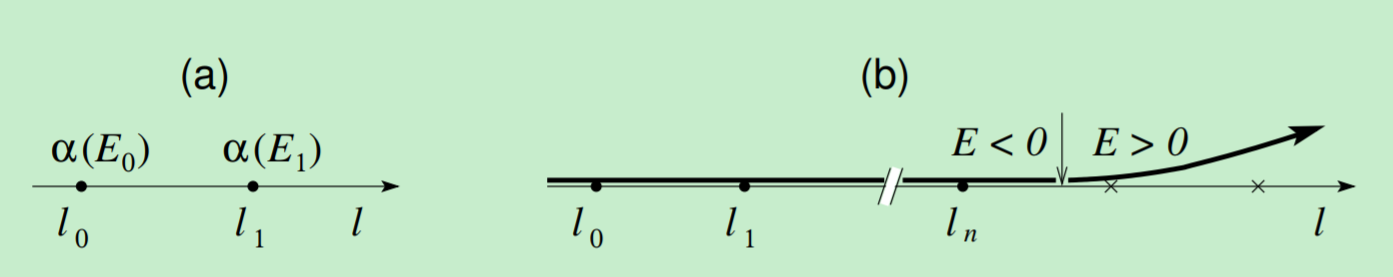
\includegraphics[scale=1]{6_8.PNG}
    \captionsetup{font={Large}}
    \caption{Regge trajectory: (a) Starting from a zero $l_0 = \alpha (E_0 <0)$ to the bound state with energy $E_0$ and angular momentum $l_0$, we increase $E$ until we find the next zero at $E_1> E_0$ with $\alpha (E_1) = l_0 + 1 = l_1$. If $E_1 <0$ we have found another bound state with energy E1 and angular momentum l1. (b) We continue to increase the parameter $E$ until we exceed the value 0 where the trajectory breaks away from the real $l$-axis.}
\end{figure}
\\\\
State until $l = 3$ can bind (for example, 3D-well or Yukawa potential) is shown in figure 6.9.
%图 6.9
\begin{figure}[ht]
    \begin{minipage}{0.5\textwidth}
        \centering
        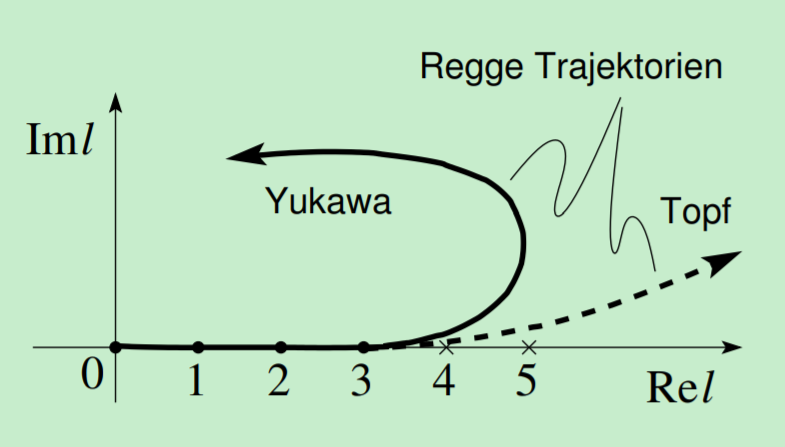
\includegraphics[scale=1]{6_9.PNG}
    \end{minipage}
    \begin{minipage}{0.5\textwidth}
        \captionsetup{font={Large}}
        \caption{Sketch of the Regge trajectories for attractive Yukawa and pot potentials which bind states up to $l = 3$ and two resonances for
        $l = 4, 5$ (pot potential).}
    \end{minipage}
\end{figure}
We can combine the two formulations in $E$ and in $l$ also for the resonances: Let $s_{l_r + il_i} (E> 0) = \infty$ for $p_r\in\mathbb{N}^0$ and $l_i$ be small. We now go to 0 with $l_i$ and follow the pole in the complex $E$-plane: the pole of $s_l$ then slides into the lower half-plane, into the 2nd Riemann plane of $E$.
\\\\
The Regge analysis allows us to define families of bound states and resonances: each RT defines a family. In the following example, the Coulomb potential, these states are represented by the states $1s, 2p, 3d, 4f,\cdots$without zeros, $n - l - 1 = 0$, by the states $2s, 3p, 4d, 5f , \cdots$ Is given with a zero, $n - l - 1 = 1$, and so on.

\section{Coulomb potential}
The fact that the Coulomb potential is a peculiarity already reveals the bound states. We compare the radial functions for the attractive Coulomb potential (with the Laguerre polynomial $\propto r^{n-1}$) and the 3D pot at $r \rightarrow\infty$,
%公式
$$
\begin{array}{cc}{\text { Coulomb }} & {3 \mathrm{D} \text { -Topf }} \\ {\qquad \underbrace{r^{n-1}}_{\text {Laguerre Polynom }} e^{-\kappa r},} & {R(r) \sim r^{-1} e^{-\kappa r}}\end{array}
$$
The expression for the Coulomb potential can be given in the generic form
%公式 98
\begin{equation}
    R_{C}(r) \sim \frac{1}{r} e^{-\kappa r+n \ln r}
    \end{equation}
with the usual asymptotic $¨ \sim exp (-\kappa r) / r$, if we make a logarithmic correction in the exponent; the above expression holds for bound states with energies $E <0$. We extrapolate (6.98) into the range of positive energies $E> 0$ by taking the quantum number n by means of the expression for the energy, $¨ E = -me^4 / 2 \sim 2\hbar^2n^2 = - \hbar^2\kappa^2 / 2m$, print by the wavenumber $\kappa$,
%公式 99
\begin{equation}
    n=\frac{m e^{2}}{\hbar^{2} \kappa}=\frac{e^{2}}{\hbar} \frac{m}{\hbar \kappa}
    \end{equation}
and then the substitutions

%公式 100
\begin{equation}
    \kappa \rightarrow-i k, \quad \frac{\hbar \kappa}{m} \rightarrow-\frac{i \hbar k}{m}=-i v, \quad n \rightarrow-i \gamma=\frac{i e^{2}}{\hbar v}=\frac{i}{a_{B} k}
    \end{equation}
make. This gives us the asymptotic for the radial function of the scattering problem
%公式 101
\begin{equation}
    R_{C}(r) \sim \frac{1}{r} e^{i(k r-\gamma \ln r)}
    \end{equation}
The comparison with (6.58) leads to the scattering phase $\delta_l\sim -\gamma \text{ln } r = (e^2 / \hbar v) \text{ln } r> 0$; as expected for an attractive potential, $\delta_l> 0$. Also, the scattering phase never becomes constant, but increases as $ -\gamma \text{ln } r$ for $r \rightarrow \infty$; the wave never becomes free (that is, it never takes the form $e^{ikr }/ r$) how far away from $r = 0$ we go too. This is a consequence of the long range of the Coulomb potential. If we replace the Coulomb potential $V_C\sim 1 / r$ by a short-range interaction (for example, via shielding: $V \sim e^{-r / \lambda} / r$ for $r\rightarrow\infty$) we obtain the asymptotic freedom of $\Psi$. In the sequence we solve the Coulomb problem first in parabolic, then in spherical coordinates.

\subsection{Coulomb Scattering Problem: Parabolic Coordinates}
Parabolic coordinates are defined as follows (see Fig. 6.10)
%公式 102
\begin{equation}
\begin{aligned} \xi &=r-z=r(1-\cos \theta) \\ \eta &=r+z=r(1+\cos \theta) \\ \varphi &=\varphi \end{aligned}
\end{equation}
The Coulomb problem in parabolic coordinates has the form
%图 6.10
\begin{figure}[ht]
    \begin{minipage}{0.5\textwidth}
        \centering
        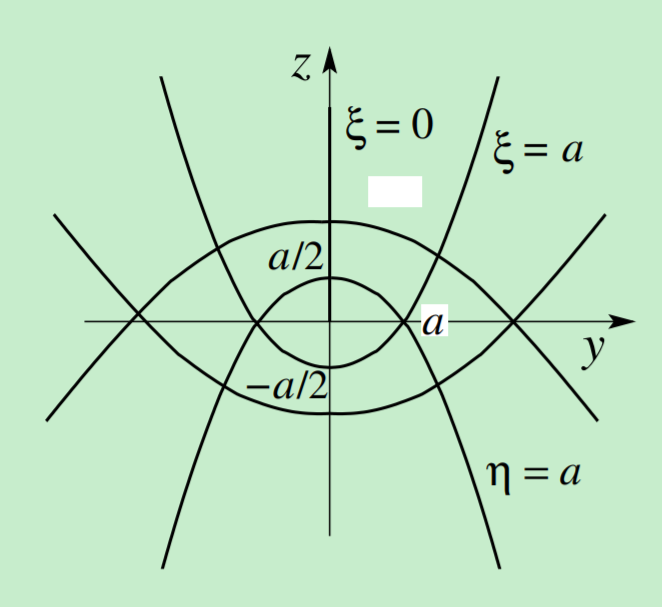
\includegraphics[scale=1]{6_10.PNG}
    \end{minipage}
    \begin{minipage}{0.5\textwidth}
        \captionsetup{font={Large}}
        \caption{Parabolic coordinates $\xi = r - z, \eta = r + z$, and azimuthal angle $\phi$. We choose $x = 0$     and $r=\sqrt{y^2+z^2}$.}
    \end{minipage}
\end{figure}

%公式 103
\begin{equation}
\begin{aligned}-\frac{\hbar^{2}}{2 m_{e}}\left[\frac{4}{\xi+\eta}\left[\partial_{\xi}\left(\xi \partial_{\xi}\right)+\partial_{\eta}\left(\eta \partial_{\eta}\right)\right]+\frac{1}{\xi \eta} \partial_{\varphi}^{2}\right] \Psi \\-\frac{2 e^{2}}{\xi+\eta} \Psi &=E \Psi \end{aligned}
\end{equation}
For the scattering problem with positive energies $¨E = \hbar^2k^2 / 2m$ we choose $\vec{k}_{in}||\hat{z}$, then for symmetry reasons $\partial_{\varphi}\Psi = 0$ and $\Psi=\Psi(\xi,\eta)$. Next we separate the incident wave $e^{ikz}$,
%公式 104
\begin{equation}
    \Psi=e^{i k z} \psi(\xi, \eta)
    \end{equation}
asymptotically we have to be $\Psi\sim e^{ikr} / r \sim e^{ikz}e^{ik\xi} / \xi$ and we make the approach $\Psi (\xi, \eta) = w (\xi)$. The differential equation for $¨w$ then results from (6.103) and we obtain the expression (the value $\gamma = e^2 /\hbar v= 1 / a_Bk$ with $v = \hbar k / m$ results for the repulsive Coulomb potential, for the Attractive potential can be found $\gamma = -e^2 / \hbar v$)

%公式 105
\begin{equation}
    \left[\xi \partial_{\xi}^{2}+(1-i k \xi) \partial_{\xi}-\gamma k\right] w(\xi)=0
    \end{equation}
The comparison with the confluent hypergeometric differential equation
%公式 106
\begin{equation}
    z \partial_{z}^{2} F+(b-z) \partial_{z} F-a F=0
    \end{equation}
with the (in $z = 0$) regular solutions (see (5.60))
%公式 107
\begin{equation}
\begin{aligned} F(a, b ; z) &=1+\frac{a}{b 1 !} z+\frac{a(a+1)}{b(b+1) 2 !} z^{2}+\cdots \\ &=\sum_{s=0}^{\infty} \frac{\Gamma(a+s) \Gamma(b)}{\Gamma(a) \Gamma(b+s) \Gamma(1+s)} z^{s} \end{aligned}
\end{equation}
shows that Equation (6.105) is the regular solution in $\xi = 0$
%公式 108
\begin{equation}
    F(-i \gamma, 1 ; i k \xi)
    \end{equation}
\footnote{Alternatively, starting from (6.103), use the separation approach $\Psi=f(\xi)g(\eta)\Phi(\varphi)$ with the separation variables $m, ν_g, ν_f$ (we simplify$ m_ee^2/\hbar^2=1/a_B,m_eE/2\hbar^2=k^2 / 4$, the $\varphi$-problem has the trivial solution $\Phi(\varphi)=e^{im\varphi}/\sqrt{2\pi}$) 

%公式 109
\begin{equation}
\begin{array}{l}{\left[\partial_{\xi}\left(\xi \partial_{\xi}\right)-\left(\frac{m^{2}}{4 \xi}-\frac{\xi k^{2}}{4}+\nu_{f}\right)\right] f(\xi)=0} \\ {\left[\partial_{\eta}\left(\eta \partial_{\eta}\right)-\left(\frac{m^{2}}{4 \eta}-\frac{\eta k^{2}}{4}+\nu_{g}\right)\right] g(\eta)=0}\end{array}
\end{equation}
and $ν_f + ν_g = -1 / a_B$. The incidental asymptotic $\Psi\sim \operatorname{exp}(ikz)=\operatorname{exp}[ik(\eta-\xi)/2],\xi\rightarrow\infty$ requires that $g (\eta) = \text{exp} (ik\eta / 2)$ and $f (\xi\rightarrow\infty) \sim \text{exp} (- ik\xi / 2)$. The approach for $g (\eta)$ defines the parameter $ν_g = ik / 2$ and the approach $f (\xi) = \text{exp} (-ik\xi / 2) w (\xi)$ leads to (6.105). The formulation of the Coulomb problem via (6.109) can also be used for the description of bound states in the attractive potential with $E = - \hbar^2\kappa^2 / 2m_e <0$. For this, one considers the asymptotic of $¨f$ (and $g$ as well) for small and large arguments with the approach $f (\xi) = \text{exp} (-\kappa\xi / 2) \xi^{| m | / 2} p (\xi)$. The resulting confluent hypergeometric differential equation is solved by the corresponding kh function $F (-n\xi, ​​| m | + 1; \kappa\xi)$ with integer parameter $n_{\xi}\geq$ solved, see Landau Lifschitz.}
\\\\
The gamma function $\Gamma (z)$ has the following properties and is shown in figure 6.11:
%公式 110
\begin{equation}
\begin{aligned} 
\Gamma(z) & \equiv \int_{0}^{\infty} d x x^{z-1} e^{-x} \\ \Gamma(1) &=\Gamma(2)=1 \\ 
\Gamma(z+1) &=z \Gamma(z) \\ 
\Gamma(n+1) &=n ! \text { for } n \geq 0, \quad &\Gamma(-n)=\infty, \text { for } n \geq 0 \\ 
\Gamma(1 / 2) &=\sqrt{\pi}, \quad &\Gamma(x) \Gamma(1-x)=\pi / \sin \pi x \\ 
\Gamma(3 / 2) &=\sqrt{\pi} / 2, \quad &\Gamma\left(z^{*}\right)=\Gamma^{*}(z) \end{aligned}
\end{equation}
%图 6.11
\begin{figure}[ht]
    \begin{minipage}{0.6\textwidth}
        \centering
        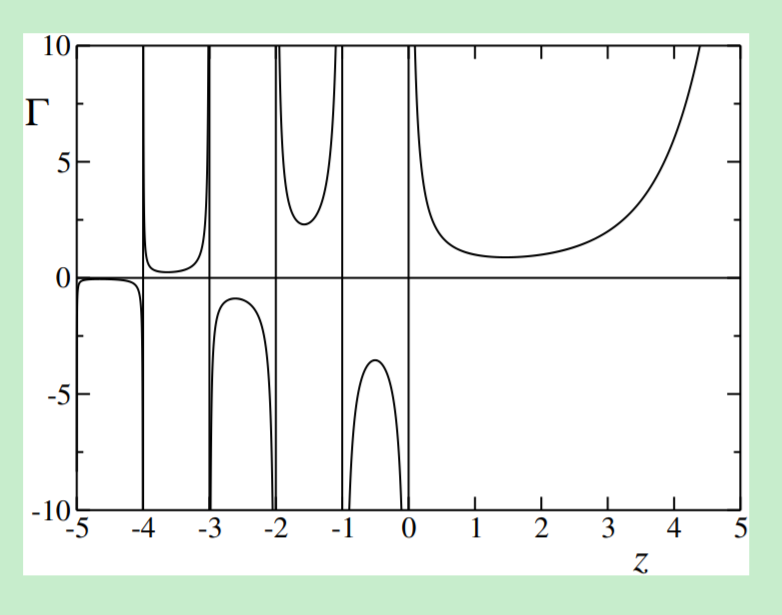
\includegraphics[scale=1]{6_11.PNG}
    \end{minipage}
    \begin{minipage}{0.4\textwidth}
        \captionsetup{font={Large}}
        \caption{Gamma function $\Gamma(z)$. For $z = n$, a natural number is $\Gamma (n + 1) = n !$; Next is $| \Gamma (-n) | = \infty, \Gamma (0) = \infty, \Gamma(1)= \Gamma(2) = 1, \Gamma (1/2) = \sqrt{\pi}, \text{ and }\Gamma (3/2) = \sqrt{\pi} / 2.$}
    \end{minipage}
\end{figure}
If we normalize the solution to $j_{in} = \hbar k / m = v$ this is the complete solution
%公式 111
\begin{equation}
    \Psi=\Gamma(1+i \gamma) e^{-\pi \gamma / 2} e^{i k z} F[-i \gamma, 1 ; i k(r-z)]
    \end{equation}
The asymptotic behavior of $F$ can be found using the integral representation (see Landau Lifschitz, Appendix $d$)

%公式 112
\begin{equation}
    F(a, b ; z)=\frac{\Gamma(b)}{2 \pi i} \int_{C} d t e^{t}(t-z)^{-a} t^{a-b}
    \end{equation}
with the integration path $C$ sketched in figure 6.12. The integrand has singularities in the points $t = z$ and $t = 0$; the path of integration is deformed corresponding to the paths $C_z$ and $C_0$ and two contributions are found
%公式 113
\begin{equation}
\begin{aligned} F(a, b ; z)=& \frac{\Gamma(b)}{\Gamma(b-a)}(-z)^{-a} g(a, a-b+1 ;-z) \\ &+\frac{\Gamma(b)}{\Gamma(a)} e^{z} z^{a-b} g(b-a, 1-a ; z) \end{aligned}
\end{equation}
With

%公式 114
\begin{equation}
    g(a, b ; z)=\frac{\Gamma(1-b)}{2 \pi i} \int_{C_{0}} d t e^{t}(1+t / z)^{-a} t^{b-1}
    \end{equation}
%图 6.12
\begin{figure}[ht]
    \begin{minipage}{0.6\textwidth}
        \centering
        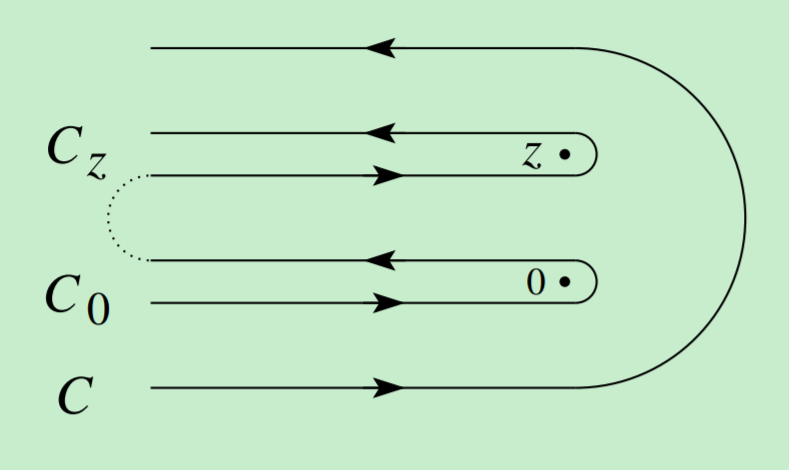
\includegraphics[scale=1]{6_12.PNG}
    \end{minipage}
    \begin{minipage}{0.4\textwidth}
        \captionsetup{font={Large}}
        \caption{Integration paths to the integral representation of $F$. The original path ¨$C$ is deformed to $C_z$ and $C_0$, where $C_z$ and $C_0$ close in the infinite (dotted line).}
    \end{minipage}
\end{figure}
The factor $(1 + t / z)^{-a}$ in $g$ can be transformed into a power series and we get the asymptotic of $g$ in the form
%公式 115
\begin{equation}
    g(a, b ; z)=1+\frac{a b}{z 1 !}+\frac{a(a+1) b(b+1)}{z^{2} 2 !}+\cdots
    \end{equation}
Applied to $F (-i\gamma, 1; ik\xi)$ we find the expression
%公式 116
\begin{equation}
\begin{aligned} 
F(-i \gamma, 1 ; i k \xi) &\sim  \frac{(-i k \xi)^{i \gamma}}{\Gamma(1+i \gamma)}\left(1+\frac{\gamma^{2}}{i k \xi}\right)+\frac{(i k \xi)^{-i \gamma} \exp (i k \xi)}{i k \xi \Gamma(-i \gamma)} \\ 
&\sim e^{\pi \gamma / 2\left[\frac{1}{\Gamma(1+i \gamma)} e^{i \gamma \ln (k \xi)}\left(1+\frac{\gamma^{2}}{i k \xi}\right)\right.} \left(1+\frac{\gamma^{2}}{i k \xi}\right) \\
&\left.+\frac{(i \gamma)}{\Gamma(1-i \gamma)} \frac{\exp (i k \xi)}{i k \xi} e^{-i \gamma \ln (k \xi)}\right] \end{aligned}
\end{equation}
where we used that $(\pm i)^{\mp i\gamma} = \text{exp} (\pi\gamma / 2)$. This gives us asymptotics for $\Psi$
%公式 117
\begin{equation}
\begin{aligned} \Psi \quad &\sim \quad \underbrace{e^{i[k z+\gamma \ln k(r-z)]}\left(1+\frac{\gamma^{2}}{i k(r-z)}\right)}_{\Psi_{\text {in }}} \\
&+\underbrace{\frac{f_{C}(\theta)}{r} e^{i(k r-\gamma \ln 2 k r)}}_{\Psi_{\text {sat }}} \end{aligned}
\end{equation}
%公式 118
\begin{equation}
\begin{aligned} \text { with } \quad f_{C}(\theta) &=-\gamma \frac{\Gamma(1+i \gamma)}{\Gamma(1-i \gamma)} \frac{e^{-i \gamma \ln \left[\sin ^{2}(\theta / 2)\right]}}{2 k \sin ^{2}(\theta / 2)} \\ &=\frac{-\gamma}{2 k \sin ^{2}(\theta / 2)} e^{-i \gamma \ln \left[\sin ^{2}(\theta / 2)\right]+2 i \delta_{0}} \end{aligned}
\end{equation}
Here, exp$ (2i\delta_0) = \Gamma (1 + i\gamma) / \Gamma (1 - i\gamma)$ and we have used that $r - z = r (1 - \text{cos} \theta) = 2r \text{sin}^2 (\theta / 2)$. The resulting cross section
%公式 119
\begin{equation}
    \frac{d \sigma_{C}}{d \Omega}=\left|f_{C}\right|^{2}=\frac{e^{4}}{16 E^{2}} \frac{1}{\sin ^{4} \theta / 2}
    \end{equation}
is identical to the classical Rutherford result and (non-integrable) singular in the forward direction $\theta = 0$, a consequence of the long-range interaction. Furthermore, the angular distribution is energy independent. (6.117) shows that the particles never become free (phase shift $\sim\gamma \text{ln} kr$), but the currents $j_{in} = \hbar k / m$ and $j_{sc} = (\hbar k / m) | f_C (\theta) |^2 / r^2$ are asymptotic well defined.

\subsection{Coulomb Scattering Problem: Sphere Coordinates}
With the approach $\Psi (r, \theta) = \Sigma_l R_{kl} (r) P_l (\text{cos}\theta)$ (note that we choose $m = 0$) we obtain the radial differential equation
%公式 120
\begin{equation}
    \left[\frac{1}{r^{2}} \partial_{r}\left(r^{2} \partial_{r}\right)+k^{2}-\frac{2 \gamma k}{r}-\frac{l(l+1)}{r^{2}}\right] R_{k l}=0
    \end{equation}
and the substitution $R_{kl} (r) = r^le^{ikr}f_{kl} (r)$ leads us to the confluent hypergeometric differential equation.\footnote{See also (5.58) and (5.61) and replace $k \rightarrow -ik, n \rightarrow -i\gamma$.}(6.106),

%公式 121
\begin{equation}
    \left\{r \partial_{r}^{2}+[2 i k r+2(l+1)] \partial_{r}+[-2 \gamma k+2 i k(l+1)]\right\} f_{k l}=0
    \end{equation}
with the solution ($C_{kl}$ the normalization constant)

%公式 122
\begin{equation}
    f_{k l}=C_{k l} F(i \gamma+l+1,2(l+1) ;-2 i k r)
    \end{equation}
For normalization we use the known solution (6.111) in the limit $r \rightarrow 0$ and obtain the asymptotic for the radial function in the form
%公式 123
\begin{equation}
    R_{k l} \sim \frac{e^{i\left(\delta_{l}+l \pi / 2\right)}}{(2 l) !} \Gamma(2 l+2) \frac{1}{k r} \sin (k r-l \pi / 2+\underbrace{\delta_{l}-\gamma \ln 2 k r}_{\text {Phasenshift }})
    \end{equation}
The scattering phases are given by
%公式 124
\begin{equation}
    e^{2 i \delta_{l}}=\frac{\Gamma(1+l+i \gamma)}{\Gamma(1+l-i \gamma)}
    \end{equation}
and determine the scattering function $f_C (\theta)$ in the partial wave analysis (The result (6.125) is equivalent to the standard result (6.49) since the expression $\Sigma_l (2l + 1) P_l (\text{cos}\theta) = 2\delta (1 - \text{cos}\theta)$ vanishes) in the singular forward direction.)
%公式 125
\begin{equation}
    f_{C}(\theta)=\frac{1}{2 i k} \sum_{l=0}^{\infty}(2 l+1) P_{l}(\cos \theta) e^{2 i \delta_{l}}
    \end{equation}
Finally, the analyticity of fC is interesting. Evidently e2iδl has poles at $l + 1 + i\gamma = 0, -1, -2, \cdots $[of $\Gamma (1 + l + i\gamma)$]. Thus, for an attractive Coulomb potential we have bound states at $k = i / na_B$, where $n = (l + 1), (l + 2), (l + 3), \cdots$. For the Regge analysis we can write (the upper (lower) sign holds for an attractive (repulsive) Coulomb potential)
%公式 126
\begin{equation}
    l=\alpha(E)=-p-i \gamma=-p \pm \frac{i m e^{2}}{\hbar^{2} k}, p \in\{1,2,3, \cdots\}
    \end{equation}
%公式 127
\begin{equation}
=\left\{\begin{array}{ll}{-p \pm\left(e^{2} / \hbar\right) \sqrt{m / 2|E|}} & {, \quad E<0} \\ {-p \pm\left(i e^{2} / \hbar\right) \sqrt{m / 2 E}} & {, \quad E>0}\end{array}\right.
\end{equation}
%图 6.13
\begin{figure}[ht]
        \centering
        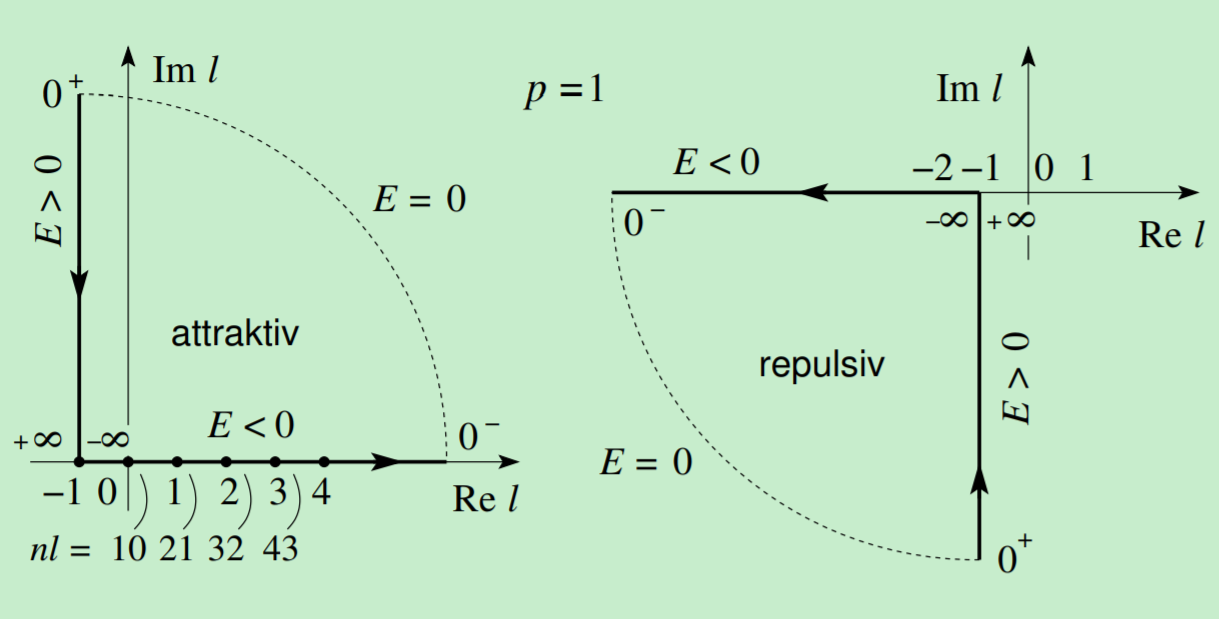
\includegraphics[scale=1]{6_13.PNG}
        \captionsetup{font={Large}}
        \caption{Regge analysis for the attractive (left) and repulsive (right) Coulomb potential. The attractive potential has bound states for all $l \in \mathbb{N}^0$ to $l = \infty$; the repulsive potential has neither bound states nor resonances}
\end{figure}
\\\\
With $p = 1$, in an attractive case we create the bound states $nl = 10, 21, 32, \cdots$. They go to$ E = 0^-$, that is, because of the long range of the Coulomb potential, we have no resonances, only bound states, for all $l\in\mathbb{N}^0$ to $l = \infty$. Thus, the Regge trajectory for $¨E \rightarrow 0^-$ runs to $\mathbb{R}^+$ infinity. For $¨P = 2$, we generate the family $20, 31, 42, \cdots$. The repulsive Coulomb problem has neither bound states nor resonances.